% CVPR 2025 Paper Template; see https://github.com/cvpr-org/author-kit

\documentclass[10pt,twocolumn,letterpaper]{article}

%%%%%%%%% PAPER TYPE  - PLEASE UPDATE FOR FINAL VERSION
% \usepackage{cvpr}              % To produce the CAMERA-READY version
% \usepackage[review]{cvpr}      % To produce the REVIEW version
\usepackage[pagenumbers]{cvpr} % To force page numbers, e.g. for an arXiv version

% Import additional packages in the preamble file, before hyperref
% \usepackage{amsmath}
% \usepackage{amssymb}
\usepackage{graphicx}
\usepackage{mathtools}
% \mathtoolsset{showonlyrefs}
\usepackage{amsfonts}
% \usepackage{amsthm,bm}
\usepackage{color}
% \usepackage{enumitem}
\usepackage{dsfont}
% \usepackage{pgfplots}
% \pgfplotsset{width=10cm,compat=1.9}
%  \usepackage{pifont}%http://ctan.org/pkg/pifont
\usepackage{thmtools} 
% \usepackage{thm-restate}
% \usepackage{sidecap}

\declaretheorem[name=Theorem]{thm}
\declaretheorem[name=Proposition]{prop}
\declaretheorem[name=Corollary]{cor}


\newcommand{\cmark}{\ding{51}}%
\newcommand{\xmark}{\ding{55}}%
\newcommand{\R}{\mathbb{R}}
\newcommand{\upmark}{\ding{218}}
\newcommand{\downmark}{\ding{216}}
\newcommand{\norm}[1]{\lVert#1\rVert}
\newcommand{\dotprod}[1]{\langle #1\rangle}
\newcommand{\E}{\mathbb{E}} 
\newcommand{\Et}[1]{\mathbf{E}_t\left[#1\right] } 
\newcommand{\Ev}[1]{\mathbf{E}_v\left[#1\right] } 
\newcommand{\EE}[2]{\mathbf{E}_{#1}\left[#2\right] } 
\newcommand{\Prb}[1]{\mathbf{P}\left[#1\right] }
\newcommand{\Tr}[1]{\mathrm{Tr}( #1)}
\newcommand{\Rea}[1]{\mathrm{Re}[ #1]}
\newcommand{\Ima}[1]{\mathrm{Im}[ #1]}
\newcommand{\eqdef}{\overset{\text{def}}{=}} 
\newcommand{\floor}[1]{\lfloor #1 \rfloor}
\newcommand{\Cov}[1]{\mathrm{Cov}\left[#1\right]}
\newcommand{\Var}[1]{\mathrm{Var}\left[#1\right]}
%\newcommand{\argmin}[1]{\underset{#1}{\text{argmin }}  } 
\newcommand{\breg}[2]{\mathcal{D}_{\Phi}\left(#1,#2\right) }
\newcommand{\xx}{\mathbf{x}}
\newcommand{\yy}{\mathbf{y}}
\newcommand{\zz}{\mathbf{z}}
\newcommand{\hmu}{\hat{\mu}}
\renewcommand{\phi}{\varphi}

%\usepackage{algorithm}
%\usepackage[noend]{algpseudocode}

\newcommand{\carles}[1]{{\color{red}{\bf[Carles:} #1{\bf]}}}
\newcommand{\ricky}[1]{{\color{magenta}{\bf[Ricky:} #1{\bf]}}}
\newcommand{\brian}[1]{{\color{orange}{\bf[Brian:} #1{\bf]}}}

% \newcommand{\carles}[1]{}
% \newcommand{\ricky}[1]{}
% \newcommand{\brian}[1]{}

\setlength{\parskip}{0.5em}
\setlength\parindent{0pt}

\graphicspath {{figures/}}

\newcommand{\N}{\mathbb{N}}
\newcommand{\Ff}{\mathcal{F}}
\newcommand{\Gg}{\mathcal{G}}
\usepackage{hyperref}
\usepackage{caption}
\usepackage[super]{nth}
\delimitershortfall-1sp

\newtheorem{lemma}{Lemma}
\newtheorem{definition}{Definition}
\newtheorem{theorem}{Theorem}
\newtheorem{note}{Note}
\newtheorem{assumption}{Assumption}
\newtheorem{proposition}{Proposition}
\newtheorem{example}{Example}
\newtheorem{remark}{Remark}
\newtheorem{corollary}{Corollary}
\newtheorem{observation}{Observation}
% \newtheorem{algorithm}{Algorithm}
\usepackage{subcaption}
%\newcommand{\corollaryautorefname}{Corollary}

\DeclareMathOperator*{\argmin}{argmin}
\DeclareMathOperator*{\argmax}{argmax}

\DeclarePairedDelimiter\abs{\lvert}{\rvert}

\renewcommand{\sectionautorefname}{Sec.}
\renewcommand{\subsectionautorefname}{Subsec.}
\renewcommand{\appendixautorefname}{App.}
\renewcommand{\theoremautorefname}{Thm.}
\renewcommand{\propositionautorefname}{Prop.}
\renewcommand{\corollaryautorefname}{Cor.}
% \renewcommand(\algorithmautorefname}{Alg.}

\newenvironment{talign*}
 {\let\displaystyle\textstyle\csname align*\endcsname}
 {\endalign}
\newenvironment{talign}
 {\let\displaystyle\textstyle\csname align\endcsname}
 {\endalign}

\makeatletter
\renewcommand{\thealgorithm}{\arabic{algorithm}}
% \@addtoreset{algorithm}{chapter}  % Remove or modify this line if you do not want to reset with chapters
\makeatother

\makeatletter
\DeclareRobustCommand{\cev}[1]{%
  {\mathpalette\do@cev{#1}}%
}
\newcommand{\do@cev}[2]{%
  \vbox{\offinterlineskip
    \sbox\z@{$\m@th#1 x$}%
    \ialign{##\cr
      \hidewidth\reflectbox{$\m@th#1\vec{}\mkern4mu$}\hidewidth\cr
      \noalign{\kern-\ht\z@}
      $\m@th#1#2$\cr
    }%
  }%
}
\makeatother

\definecolor{mygray}{gray}{0.95}
\newcommand{\greybox}[1]{
\vspace{-0.9em}
\begin{center}			% Centering minipage
\vspace{-0.5em}
\colorbox{mygray} {		% Set's the color of minipage
\begin{minipage}{0.987\linewidth} 	% Starts minipage
\centering
\vspace{-0.8em}
{#1}
\end{minipage}}			% End minipage
\end{center}
\vspace{-0.5em}
}

% It is strongly recommended to use hyperref, especially for the review version.
% hyperref with option pagebackref eases the reviewers' job.
% Please disable hyperref *only* if you encounter grave issues, 
% e.g. with the file validation for the camera-ready version.
%
% If you comment hyperref and then uncomment it, you should delete *.aux before re-running LaTeX.
% (Or just hit 'q' on the first LaTeX run, let it finish, and you should be clear).
\definecolor{cvprblue}{rgb}{0.21,0.49,0.74}
\usepackage[pagebackref,breaklinks,colorlinks,allcolors=cvprblue]{hyperref}
% \usepackage{cleveref}
\usepackage{verbatim}

\usepackage{wrapfig}  % Add this to your preamble
\usepackage{graphicx}
\usepackage{floatrow}
\usepackage{subcaption}
\usepackage{listings}
\usepackage{algorithm}

%%%%%%%%% PAPER ID  - PLEASE UPDATE
\def\cvprPaperID{163} % *** Enter the Paper ID here
\def\confName{CVPR}
\def\confYear{2025}

%----------------------------------------------------------
% define pseudo-code style
\lstset{
  backgroundcolor=\color{white},
  basicstyle=\fontsize{7.5pt}{7.5pt}\ttfamily\selectfont,
  columns=fullflexible,
  breaklines=true,
  captionpos=b,
  commentstyle=\fontsize{7.5pt}{7.5pt}\color{codeblue},
  keywordstyle=\fontsize{7.5pt}{7.5pt}\color{codekw},
}
%----------------------------------------------------------

%%%%%%%%% TITLE - PLEASE UPDATE
\title{Causal Diffusion Transformers for Generative Modeling}

%%%%%%%%% AUTHORS - PLEASE UPDATE
\author{Chaorui Deng ~~~~ Deyao Zhu ~~~~ Kunchang Li ~~~~ Shi Guang ~~~~ Haoqi Fan\\
ByteDance Research\\
\tt\small{\href{https://github.com/causalfusion/causalfusion.git}{https://github.com/causalfusion}} \\
% For a paper whose authors are all at the same institution,
% omit the following lines up until the closing ``}''.
% Additional authors and addresses can be added with ``\and'',
% just like the second author.
% To save space, use either the email address or home page, not both
}



\begin{document}
\maketitle
\begin{abstract}
We introduce Causal Diffusion as the autoregressive (AR) counterpart of Diffusion models. It is a next-token(s) forecasting framework that is friendly to both discrete and continuous modalities and compatible with existing next-token prediction models like LLaMA and GPT. While recent works attempt to combine diffusion with AR models, we show that introducing sequential factorization to a diffusion model can substantially improve its performance and enables a smooth transition between AR and diffusion generation modes. Hence, we propose \textbf{CausalFusion} - a decoder-only transformer that dual-factorizes data across sequential tokens and diffusion noise levels, leading to state-of-the-art results on the ImageNet generation benchmark while also enjoying the AR advantage of generating an arbitrary number of tokens for in-context reasoning. We further demonstrate CausalFusion's multimodal capabilities through a joint image generation and captioning model, and showcase CausalFusion's ability for zero-shot in-context image manipulations. We hope that this work could provide the community with a fresh perspective on training multimodal models over discrete and continuous data.
\end{abstract}
\vspace{-10pt}
\section{Introduction}
\label{sec:intro}
Autoregressive (AR) and diffusion models are two powerful paradigms for data distribution modeling. AR models, also known as the next token prediction approach, dominate language modeling and are considered central to the success of large language models (LLMs)~\cite{gpt1,gpt2,gpt3,llama1,llama2,llama3}. On the other hand, diffusion models~\cite{ddpm,dit,adm,edm}, or score-based generative models~\cite{songscore,lipman2023flow}, have emerged as the leading approach for visual generation, driving unprecedented progress in the era of visual content generation~\cite{sora,rombach2022high,li2023scaling}. 

\begin{figure}[t]
    \centering
    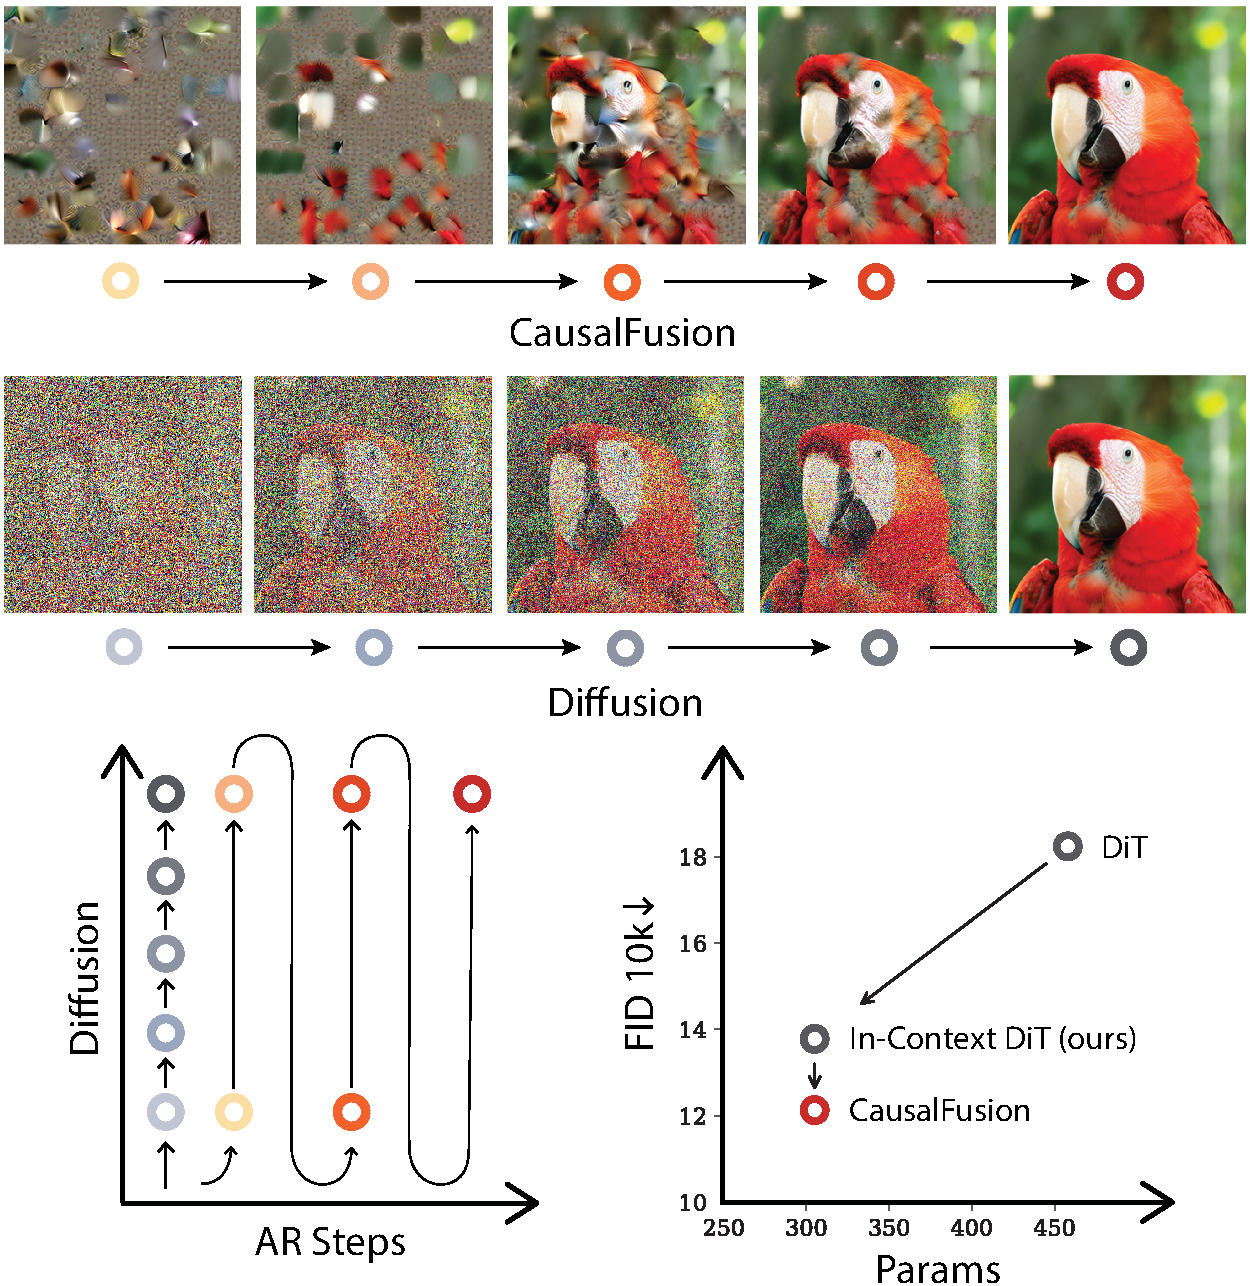
\includegraphics[width=1.0\textwidth,height=1.0\textwidth]{figs/casualfusion-teaser-v6.pdf} 
    \vspace*{-6mm}
    \caption{
    \textbf{Illustration of Dual-Factorization}. The arrow line indicates CausalFusion's generation path, moving from one state to the next by jointly generating along the sequential and noise-level dimension at each step. 
    Compared to DiT, our In-context DiT substantially improves results with fewer parameters. CausalFusion further enhances performance without changing the architecture or parameter count. Results were trained on IN1K for 240 epochs. CausalFusion adopts arbitrary AR steps for image generation, but each step only diffuses partial tokens, resulting in similar (or slightly lower) computational complexity.
    \vspace{-10pt}
    }
    \label{fig:dual-factorization}
\end{figure}


\begin{figure*}[t]
  \centering
  \begin{subfigure}{1.0\linewidth}
    \centering
    \includegraphics[width=\linewidth]{figs/figure2.pdf}
    \caption{Samples generated by CausalFusion-XL/2, ImageNet 512$\times$512, 800 epoch, DDPM 250 steps, CFG=4.0}
  \end{subfigure}
  \begin{subfigure}{1.0\linewidth}
    \centering
    \includegraphics[width=\linewidth]{figs/edit.pdf}
    \caption{\textbf{Zero-shot image editing} results generated by CausalFusion-XL/2, ImageNet 512$\times$512, 800 epoch. We first generate the original image (those on the left), then mask out its centre region, top-half, or bottom-half, and regenerate the image with new class conditions. Details are discussed in Sec \ref{sec:system}.}
  \end{subfigure}
  \caption{\textbf{Visualization results}. All samples are generated by models trained only on \textbf{ImageNet-1K class-conditional generation} task, demonstrating CausalFusion's zero-shot image manipulation ability. See more visualization results in Appendix~\ref{appendix:secD}.
  \vspace{-12pt}
  }
  \vspace{-6pt}
  \label{fig:vis1}
\end{figure*}

The intrinsic distinction between AR and diffusion models lies in their approach to data distribution factorization. AR models treat data as an ordered sequence, factorizing it along the sequential axis, where the probability of each token is conditioned on all preceding tokens. This factorization enables the AR paradigm to generalize effectively and efficiently across arbitrary number of tokens, making it well-suited for long-sequence reasoning and in-context generation. In contrast, diffusion models factorize data along the noise-level axis, where the tokens at each step are a refined (denoised) version of themselves from the previous step. As a result, the diffusion paradigm is generalizable to arbitrary number of data refinement steps, enabling iterative quality improvement with scaled inference compute. While AR and diffusion models each excel within their respective domains, their distinct factorization approaches reveal complementary potential. Although recent studies~\cite{transfusion,monoformer,dart} have attempted to integrate AR and diffusion within a single model, they typically treat these paradigms as separate modes, missing the potential benefits of jointly exploring them within a 2-D factorization plane.

To this end, we introduce \textbf{CausalFusion}, a flexible framework that integrates both sequential and noise-level data factorization to unify their advantages. The degree of factorization along these two axes—namely, the AR step and diffusion step—is adjustable, enabling {CausalFusion} to revert seamlessly to the traditional AR or diffusion paradigms at either extreme. To enhance its generality, CausalFusion is designed to predict \textit{any} number of tokens at \textit{any} AR step, with \textit{any} pre-defined sequence order and \textit{any} level of inference compute, thereby minimizing the inductive biases presented in existing generative models. As shown in Figure~\ref{fig:dual-factorization}, this approach provides a broad spectrum between the AR and diffusion paradigms, allowing smooth interpolation within two endpoints during both training and inference. 
Specifically, we explore CausalFusion in image generation and multimodal generation scenarios, where we observe that the level of training difficulties significantly influences the overall effectiveness of CausalFusion.

\textbf{Difficulties of generative tasks in CausalFusion:} Both AR and diffusion paradigms present unique challenges based on difficulties of their specific generative stages. In diffusion models, the effectiveness of training depends heavily on proper loss weighting across noise levels~\cite{ddpm,minsnr}, as higher noise levels are more difficult and usually provide more valuable signals than lower noise levels. Similarly, AR models are susceptible to error accumulation~\cite{bengio2015scheduled} as early-stage predictions are made with limited visible context, making them more error-prone. Optimizing CausalFusion thus requires balancing across these varying task difficulties to optimize training signal impact and ensure sufficient exploration across the entire factorization plane.

In this paper, we formally examine the difficulties of generative tasks within CausalFusion. We show that, in addition to the noise levels in diffusion and the amount of visible context in AR, the total number of AR steps, which controls the interpolation between AR and diffusion, also plays a critical role in shaping training difficulties. Driven by these factors, we develop a scalable and versatile model based on the CausalFusion framework. Starting from the DiT architecture~\cite{dit}, we gradually convert it into a decoder-only transformer compatible with existing AR models like GPT~\cite{gpt1,gpt2,gpt3} and LLaMA~\cite{llama1,llama2,llama3}. We provide insights on how to appropriately choose the number of AR steps during the training of CausalFusion models, and further introduce loss weighing along both the diffusion and AR axis to balance the impact of different generative stages. As shown in Figure~\ref{fig:dual-factorization} and ~\ref{fig:vis1}, our model achieves state-of-the-art performance on the ImageNet class-conditional generation benchmark, significantly outperforming DiT~\cite{dit} and enabling zero-shot image manipulations due to its AR nature. When pretraining on both text-to-image and image-to-text tasks, our model surpasses forced-fusion frameworks such as TransFusion~\cite{transfusion}, demonstrating the versatility of our CausalFusion framework.


We highlight our main contribution below:
\begin{itemize}
\item  We propose CausalFusion as the AR counterpart to DiT, achieving state-of-the-art results and enabling the unlimited token generation for in-context reasoning.
\item  We systematically study CausalFusion on the dual-factorization plane and identify key factors that improve the effectiveness of CausalFusion models.
\item  Compared with recent studies~\cite{transfusion}, CausalFusion enables a smooth, cohesive integration with language modeling for cross-modal generation and reasoning.
\end{itemize} 

% \begin{figure}[t]
%   \begin{minipage}{0.49\textwidth}
%      \centering
%     \includegraphics[width=1.0\textwidth]{fig/MLMF.png}
%     \caption{Multi-Layer Motion Fusion.}
%     \label{fig: frameselector_abalation}
    
%   \end{minipage}
%   \hfill
%    \begin{minipage}{0.48\textwidth}
%     \centering
%     \includegraphics[width=0.8\textwidth]{fig/SMPL.jpg}
%     \caption{Prametric Shape Alignment.}
%     \label{fig:Visualizedselected_frames}
%   \end{minipage}
% \vspace{-3mm}
% \end{figure}


\section{Related Work}
\label{sec:related_work}

\textbf{Diffusion Models for Image Generation.}
Diffusion-based models~\cite{balaji2022ediffi,huang2023composer,nichol2021glide,ramesh2022hierarchical,rombach2022high,saharia2022photorealistic} have rapidly emerged as a fundamental component in the domain of text-to-image generation, renowned for their capacity to yield highly promising generative outcomes. 
To address the considerable computational requirements inherent in diffusion models, the Latent Diffusion Model, as proposed in~\cite{rombach2022high} introduces a technique for denoising within the latent space.
This method not only enhances the computational efficiency of these models but also preserves their ability to generate high-fidelity images.
Moreover, in the endeavor to enhance control over visual generation, recent studies such as ControlNet~\cite{zhang2023adding}, T2I-Adapter~\cite{mou2023t2i}, and IP-Adapter~\cite{ye2023ip} have delved into the incorporation of supplementary encoder layers.
These layers facilitate the assimilation of control signals encompassing aspects such as pose, depth, and edge information, and even permit the utilization of images in conjunction with textual prompts.
This progression signifies a significant advancement towards more controlled and precise image generation, facilitating the creation of images characterized by not only superior quality but also enriched contextual accuracy and detail.


\textbf{Diffusion Models for Human Image Animation.}
The task of animating human images, a significant endeavor within the domain of video generation, aims to seamlessly create videos from one or multiple static images~\cite{chan2019everybody,ren2020deep,siarohin2019first,siarohin2021motion,yu2023bidirectionally,zhang2022exploring,zhao2022thin,yoon2021pose, sarkar2021neural, hu2023sherf, albahar2023humansgd, cao2023dreamavatar, prokudin2021smplpix, fu2022styleganhuman, jiang2023humangen}.
The recent advancements of diffusion models in the text-to-image domain have sparked interest in exploring their utility for animating human images.
PIDM~\cite{bhunia2023person} introduces a texture diffusion module that is specifically crafted to align the texture patterns of the source and target images closely, thereby enhancing the realism of the resultant animated output.
DreamPose~\cite{karras2023dreampose} capitalizes on the capabilities of the pre-trained Stable Diffusion model by incorporating both CLIP~\cite{radford2021learning} and VAE~\cite{kingma2013auto} for image encoding. 
It integrates these embeddings with an adapter. 
Similarly, DisCo~\cite{wang2023disco} innovatively segregates the control of pose and background using dual independent ControlNets~\cite{zhang2023adding}, providing finer control over the animation process. 
Animate Anyone~\cite{hu2023animate} utilizes a UNet-based ReferenceNet to extract features from reference images.
It includes pose information via a lightweight pose guider. Expanding on the principles introduced by AnimateDiff~\cite{guo2023animatediff}, Animate Anyone integrates a temporal layer into the denoising UNet to enhance temporal coherence.
MagicAnimate~\cite{xu2023magicanimate} follows a similar approach but employs a ControlNet tailored for DensePose \cite{guler2018dense} inputs instead of the more commonly used OpenPose~\cite{cao2017realtime} keypoints to provide more precise pose guidance.
This paper primarily builds upon esteemed diffusion-based methodologies and advances the optimization of appearance alignment and motion guidance mechanisms. 
This is achieved by introducing a 3D parametric model for geometric reconstruction of the reference image and motion modeling of the source video sequence.


\textbf{Pose Guidance in Human Image Animation.}
DWpose\cite{yang2023effective} stands out as an enhanced alternative to OpenPose\cite{cao2017realtime}, offering more accurate and expressive skeletons. 
This improvement has proven beneficial for diffusion models in generating higher quality images, with its adoption as a condition signal in various works\cite{feng2023dreamoving,hu2023animate}.
The work presented in DensePose~\cite{Guler2018DensePose} aims to establish dense correspondences between an RGB image and a surface-based representation.
The SMPL~\cite{SMPL:2015} model is a 3D model renowned for its realistic depiction of human bodies through skinning and blend shapes.
Its widespread adoption spans fields like human reconstruction\cite{he2021arch,alldieck2018video} and interaction with environments\cite{hassan2021populating,ma2020learning}. 
It also serves as essential ground truth for neural networks in pose and shape analysis\cite{lu2023dposer,mu2023actorsnerf}.
In this paper, we consider SMPL, the 3D parametric model, to reconstruct the poses as well as the shapes from the source video, and obtain more complete condition for appearance alignment and pose guidance.

\begin{figure}[t]
  \centering
  \includegraphics[width=0.95\linewidth]{fig/framework.jpg}
  \caption{The overview of our proposed approach. Given an input human image and a reference video depicting a motion sequence. We obtain the pose sequence corresponding to the reference image through Parametric Shape Alignment as 3D motion guidance. MLMF is employed to encode multi-layer 3D-related motion information. Referencenet and Temporal-attention ensure identity consistency and temporal coherence, respectively.}
  \vspace{-6mm}
  \label{fig:network}
\end{figure}
\section{Method}
%%%%%%%%% Figure: Overall framework
\begin{figure*}[t]
  \centering
   \includegraphics[width=0.85\linewidth]{figures/PoolFormer_overall_architecture.pdf}
   \vspace{-4mm}
   \caption{\textbf{(a) The overall framework of \modelname{}.} Similar to \cite{resnet, pvt, swin}, \modelname{} adopts hierarchical architecture with 4 stages. For a model with L \modelname{} blocks, stage [1, 2, 3, 4] have [L/6, L/6, L/2, L/6] blocks, respectively. The feature dimension $D_i$ of stage $i$ is shown in the figure. \textbf{(b) The architecture of \modelname{} block.} Compared with Transformer block, it replaces attention with extremely simple non-parametric operator, pooling, to conduct only basic token mixing.}
   \label{fig:overall_architecture}
\end{figure*}


%%%%%%%%% Algorithm: Pooling
\begin{algorithm}[t]
\caption{Pooling for PoolFormer, PyTorch-like Code}
\label{alg:code}
\definecolor{codeblue}{rgb}{0.25,0.5,0.5}
\definecolor{codekw}{rgb}{0.85, 0.18, 0.50}
\lstset{
  backgroundcolor=\color{white},
  basicstyle=\fontsize{7.5pt}{7.5pt}\ttfamily\selectfont,
  columns=fullflexible,
  breaklines=true,
  captionpos=b,
  commentstyle=\fontsize{7.5pt}{7.5pt}\color{codeblue},
  keywordstyle=\fontsize{7.5pt}{7.5pt}\color{codekw},
}
\begin{lstlisting}[language=python]
import torch.nn as nn

class Pooling(nn.Module):
    def __init__(self, pool_size=3):
        super().__init__()
        self.pool = nn.AvgPool2d(
            pool_size, stride=1, 
            padding=pool_size//2, 
            count_include_pad=False,
        )
    def forward(self, x):
        """
        [B, C, H, W] = x.shape
        Subtraction of the input itself is added 
        since the block already has a 
        residual connection.
        """
        return self.pool(x) - x
\end{lstlisting}
\end{algorithm}

\subsection{MetaFormer}
We present the core concept ``MetaFormer" for this work at first. As shown in Figure \ref{fig:first_figure}, abstracted from Transformers \cite{transformer}, 
MetaFormer is a general architecture where the token mixer is not specified while the other components are kept the same as Transformers. The input $I$ is first processed by input embedding, such as  patch embedding for ViTs \cite{vit},
\begin{equation}
    X = \mathrm{InputEmb}(I),
\end{equation}
where  $X \in \mathbb{R}^{N \times C}$ denotes the embedding tokens with sequence length $N$ and embedding dimension $C$. 


Then, embedding tokens are fed to repeated MetaFormer blocks, each of which includes two residual sub-blocks. Specifically, the first sub-block mainly contains a token mixer to communicate information among tokens and this sub-block can be expressed as
\begin{equation}
    Y = \mathrm{TokenMixer}(\mathrm{Norm}(X)) + X,
\end{equation}
where $\mathrm{Norm}(\cdot)$ denotes the normalization such as Layer Normalization \cite{layer_norm} or Batch Normalization \cite{batch_norm}; $\mathrm{TokenMixer}(\cdot)$ means a module mainly working for mixing token information. It is implemented by various attention mechanism in recent vision Transformer models  \cite{vit,refiner,t2t} or spatial MLP in MLP-like models \cite{mlp-mixer, resmlp}. Note that the main function of the token mixer is to propagate token information although some token mixers can also mix channels, like attention. 


The second sub-block primarily consists of a two-layered MLP with non-linear activation, 
\begin{equation}
    Z = \sigma(\mathrm{Norm}(Y)W_1)W_2 + Y,
\end{equation}
where $W_1 \in \mathbb{R}^{C \times rC}$ and $W_2 \in \mathbb{R}^{rC \times C}$ are learnable parameters with MLP expansion ratio $r$; $\sigma(\cdot)$ is a non-linear activation function, such as GELU \cite{gelu} or ReLU \cite{relu}. 

\myPara{Instantiations of MetaFormer} MetaFormer describes a general architecture 
% a general architecture that is powerful at solving computer vision tasks.  
with which different models can be obtained immediately by specifying the concrete design of the token mixers. 
As shown in Figure \ref{fig:first_figure}(a), if the token mixer is specified as attention or spatial MLP, MetaFormer then becomes a Transformer or MLP-like model respectively. 

\subsection{PoolFormer}
From the introduction of Transformers \cite{transformer}, lots of works attach much importance to the attention and focus on designing various attention-based token mixer components. In contrast, these works pay little attention to the general architecture, \ie, the MetaFormer.


In this work, we argue that this MetaFormer general architecture contributes mostly to the success of the recent Transformer and MLP-like models. 
To demonstrate it, we deliberately employ an embarrassingly simple operator, pooling, as the token mixer. This operator has no learnable parameters and it just makes each token averagely aggregate its nearby token features. 


Since this work is targeted at vision tasks,  we assume the input is in channel-first data format, \ie,  $T \in \mathbb{R}^{C \times H \times W}$. The pooling operator can be expressed as
\begin{equation}
\label{eq:pool}
    T'_{:, i, j} =  \frac{1}{K \times K} \sum_{p,q=1}^{K}T_{:, i+p-\frac{K+1}{2}, i+q-\frac{K+1}{2}} - T_{:, i, j},
\end{equation}
where $K$ is the pooling size. Since the MetaFormer block already has a residual connection, subtraction of the input itself is added in Equation (\ref{eq:pool}). The PyTorch-like code of the pooling is shown in Algorithm \ref{alg:code}.


As well known, self-attention and spatial MLP have computational complexity quadratic to the number of tokens to mix. Even worse, spatial MLPs bring much more parameters when handling longer sequences. As a result, self-attention and spatial MLPs usually can only process hundreds of tokens. In contrast, the pooling needs a computational complexity linear to the sequence length without any learnable parameters.  Thus, we take advantage of pooling by adopting a hierarchical structure similar to traditional CNNs \cite{alexnet, vgg, resnet} and recent hierarchical Transformer variants \cite{swin, pvt}. Figure \ref{fig:overall_architecture} shows the overall framework of PoolFormer. Specifically, PoolFormer has 4 stages with $\frac{H}{4} \times \frac{W}{4}$, $\frac{H}{8} \times \frac{W}{8}$, $\frac{H}{16} \times \frac{W}{16}$, and $\frac{H}{32} \times \frac{W}{32}$ tokens respectively, where $H$ and $W$ represent the width and height of the input image. There are two groups of embedding size: 1) small-sized models with embedding dimensions of 64, 128, 320, and 512 responding to the four stages; 2) medium-sized models with embedding dimensions 96, 192, 384, and 768. Assuming there are $L$ PoolFormer blocks in total, stages 1, 2, 3, and 4 will contain $L/6$, $L/6$, $L/2$, and $L/6$ PoolFormer blocks respectively. The MLP expansion ratio is set as 4. According to the above simple model scaling rule, we obtain 5 different model sizes of PoolFormer and their hyper-parameters are shown in Table \ref{tab:model}.


%%%%%%%%% Table: Model Configurations
\begin{table}[t]
\footnotesize
\centering
\setlength{\tabcolsep}{2pt}
% \scalebox{0.65}{\newcommand{\blockc}[4]{
$\begin{bmatrix}
	\begin{array}{l}
	R_1=#1 \\
	N_1=#2 \\
	E_1=#3 \\
	\end{array}
\end{bmatrix} \times #4$
}

\newcommand{\sblock}[3]{
$\begin{matrix}
E_{#1}=#2 \\
L_{#1}=#3 \\
\end{matrix}$
}

\newcommand{\poollayer}{
Pooling Size & \multicolumn{5}{c}{$3 \times 3$, stride 1}\\
\cline{4-9}
}

\newcommand{\stitle}[6]{
\multirow{5}{*}{#1} & \multirow{5}{*}{\scalebox{1}{$\frac{H}{#2}\times \frac{W}{#2}$}} & \multirow{2}{*}{\tabincell{c}{Patch \\ Embedding}} & Patch Size & \multicolumn{5}{c}{$#3 \times #3$, stride $#4$} \\
\cline{4-9}
    &    &    & Embed. Dim. & \multicolumn{3}{c|}{$#5$} & \multicolumn{2}{c}{$#6$} \\
\cline{3-9}
& & \multirow{3}{*}{\tabincell{c}{\modelname{}\\Block}} 
}

\begingroup
\renewcommand{\arraystretch}{1.1}
\begin{tabular}{c|c|c|c|c|c|c|c|c}
\toprule
  \multirow{2}{*}{Stage} & \multirow{2}{*}{\#Tokens} & \multicolumn{2}{c|}{\multirow{2}{*}{Layer Specification}} & \multicolumn{5}{c}{\modelname{}} \\
\cline{5-9}
 & & \multicolumn{2}{c|}{} & S12 & S24 & S36 & M36 & M48 \\
\whline
\stitle{1}{4}{7}{4}{64}{96}    & \poollayer
 & & & MLP Ratio & \multicolumn{5}{c}{4} \\
\cline{4-9}
 & & & \# Block & 2 & 4 & 6 & 6 & 8 \\
\hline
\stitle{2}{8}{3}{2}{128}{192}  & \poollayer
 & & & MLP Ratio & \multicolumn{5}{c}{4} \\
 \cline{4-9}
 & & & \# Block & 2 & 4 & 6 & 6 & 8 \\
\hline
\stitle{3}{16}{3}{2}{320}{384} & \poollayer
 & & & MLP Ratio & \multicolumn{5}{c}{4} \\
\cline{4-9}
 & & & \# Block & 6 & 12 & 18 & 18 & 24 \\
\hline
\stitle{4}{32}{3}{2}{512}{768} & \poollayer
 & & & MLP Ratio & \multicolumn{5}{c}{4} \\
 \cline{4-9}
 & & & \# Block & 2 & 4 & 6 & 6 & 8 \\
\hline
\multicolumn{4}{c|}{Parameters~(M)}& 11.9 & 21.4              &  30.8            &  56.1              &  73.4    \\
\hline
\multicolumn{4}{c|}{MACs~(G)}     & 1.8  &  3.4              &  5.0             &  8.8              &  11.6    \\
\bottomrule
\end{tabular}
\endgroup
}
\newcommand{\blockc}[4]{
$\begin{bmatrix}
	\begin{array}{l}
	R_1=#1 \\
	N_1=#2 \\
	E_1=#3 \\
	\end{array}
\end{bmatrix} \times #4$
}

\newcommand{\sblock}[3]{
$\begin{matrix}
E_{#1}=#2 \\
L_{#1}=#3 \\
\end{matrix}$
}

\newcommand{\poollayer}{
Pooling Size & \multicolumn{5}{c}{$3 \times 3$, stride 1}\\
\cline{4-9}
}

\newcommand{\stitle}[6]{
\multirow{5}{*}{#1} & \multirow{5}{*}{\scalebox{1}{$\frac{H}{#2}\times \frac{W}{#2}$}} & \multirow{2}{*}{\tabincell{c}{Patch \\ Embedding}} & Patch Size & \multicolumn{5}{c}{$#3 \times #3$, stride $#4$} \\
\cline{4-9}
    &    &    & Embed. Dim. & \multicolumn{3}{c|}{$#5$} & \multicolumn{2}{c}{$#6$} \\
\cline{3-9}
& & \multirow{3}{*}{\tabincell{c}{\modelname{}\\Block}} 
}

\begingroup
\renewcommand{\arraystretch}{1.1}
\begin{tabular}{c|c|c|c|c|c|c|c|c}
\toprule
  \multirow{2}{*}{Stage} & \multirow{2}{*}{\#Tokens} & \multicolumn{2}{c|}{\multirow{2}{*}{Layer Specification}} & \multicolumn{5}{c}{\modelname{}} \\
\cline{5-9}
 & & \multicolumn{2}{c|}{} & S12 & S24 & S36 & M36 & M48 \\
\whline
\stitle{1}{4}{7}{4}{64}{96}    & \poollayer
 & & & MLP Ratio & \multicolumn{5}{c}{4} \\
\cline{4-9}
 & & & \# Block & 2 & 4 & 6 & 6 & 8 \\
\hline
\stitle{2}{8}{3}{2}{128}{192}  & \poollayer
 & & & MLP Ratio & \multicolumn{5}{c}{4} \\
 \cline{4-9}
 & & & \# Block & 2 & 4 & 6 & 6 & 8 \\
\hline
\stitle{3}{16}{3}{2}{320}{384} & \poollayer
 & & & MLP Ratio & \multicolumn{5}{c}{4} \\
\cline{4-9}
 & & & \# Block & 6 & 12 & 18 & 18 & 24 \\
\hline
\stitle{4}{32}{3}{2}{512}{768} & \poollayer
 & & & MLP Ratio & \multicolumn{5}{c}{4} \\
 \cline{4-9}
 & & & \# Block & 2 & 4 & 6 & 6 & 8 \\
\hline
\multicolumn{4}{c|}{Parameters~(M)}& 11.9 & 21.4              &  30.8            &  56.1              &  73.4    \\
\hline
\multicolumn{4}{c|}{MACs~(G)}     & 1.8  &  3.4              &  5.0             &  8.8              &  11.6    \\
\bottomrule
\end{tabular}
\endgroup

\vspace{-3mm}
\caption{\textbf{ Configurations of different PoolFormer models.} There are two groups of embedding dimensions, \ie, small size with [64, 128, 320, 512] dimensions and medium size with [96, 196, 384, 768]. Notation ``S24" means the model is in small size of embedding dimensions with 24 PoolFormer blocks in total. The numbers of MACs are counted by \texttt{fvcore}\cite{fvcore} library.
}
\label{tab:model}
\vspace{-4mm}
\end{table}

\section{Conclusion}
In this paper, we present~\name, a real-world VSR framework that leverages T2V diffusion prior to restore videos with fewer artifacts, higher spatial fidelity, and stronger temporal consistency. Specifically, we introduce a Local Information Enhancement Module into the original T2V backbone to improve its ability to handle degradations and reconstruct fine details. Additionally, we propose a Dynamic Frequency Loss that guides the model to focus on restoring different frequency components at each diffusion step, thereby enhancing fidelity. Furthermore, we demonstrate that a powerful T2V model can effectively generate high-quality results in both spatial and temporal dimensions. Extensive experiments show that~\name~achieves superior performance in both spatial and temporal quality. We hope our work lays a solid foundation for applying T2V models in real-world VSR and inspires future advancements in the field.
\section{Appendix} \label{appendix}


\subsection{NewYorker Data for evaluation}

\begin{figure}[!ht]
\small
\centering
\includegraphics[width=0.4\textwidth]{figures/length.png}
\caption{\label{lengthdist} Distribution of word count of stories in our test set}
\end{figure}

Table \ref{teststories} shows the data used for conducting our evaluation. The 12 stories shown are taken from The New Yorker and summarized into single-sentence plots. These stories come from highly established literary experts acting as an upper bound for what it means to be creative. These stories span complex themes.

\begin{table*}[!ht]
\centering
\small
\def\arraystretch{1.35}
\begin{tabular}{|l|}
\hline
\begin{tabular}[c]{@{}l@{}}Write a New Yorker-style story given the plot below. Make sure it is atleast \textbf{\color{blue}\{\{word\_count\}\}} words. Directly start with the\\ story, do not say things like `Here's the story {[}...{]}:\end{tabular}                                                                                                                                                                                            \\ \hline\hline
\begin{tabular}[c]{@{}l@{}}You wrote the story I gave you below. I requested a story with \textbf{\color{blue}\{\{word\_count\}\}} words, but the story only has\\ \textbf{\color{blue}\{\{current\_word\_count\}\}} words. Can you rewrite the story to make it longer, and closer to the \textbf{\color{blue}\{\{word\_count\}\}} word target\\ I gave you. Directly start with the story, do not say things like `Here's the story {[}...{]}:`\\ \\ Current story: \{\{story\}\}\end{tabular} \\ \hline
\end{tabular}
\vspace{2ex}
\caption{\label{promptstory}Prompt to write the initial story (Row1) vs Prompt to rewrite the initial story to be longer. word\_count represents the number of words in the human written story on a given plot (P) while current\_word\_count represents the number of words in the LLM generated story on the same plot (P)}
\end{table*}

\begin{table*}[!ht]
\def\arraystretch{1.15}
\small
\begin{tabular}{|l|l|}
\hline
Story                                    & Plot                                                                                                                                                                                                                                                                                                                                                                                                                                                                                                                                   \\ \hline
\href{https://www.newyorker.com/books/flash-fiction/a-triangle}{A Triangle}                               & \begin{tabular}[c]{@{}l@{}}An observer becomes entranced by a seemingly ordinary couple on the street, follows them home, and then \\watches them from outside in the rising floodwaters, drawing an eerie connection between the woman and\\ a discarded, burned chair they'd noticed earlier.\end{tabular}                                                                                                                                                                    \\ \hline\hline
\href{https://www.newyorker.com/books/flash-fiction/barbara-detroit-1966}{\begin{tabular}[c]{@{}l@{}}Barbara\\ Detroit,1966\end{tabular}}                    & \begin{tabular}[c]{@{}l@{}}On Feb 12, 1966, a heavily pregnant woman named Barbara experienced a shocking incident in her synagogue\\in Southfield, Detroit, where a young man shot and killed the renowned Rabbi Adler before turning the gun\\ on himself, and though Barbara tried to reach the shooter, she was swept away by the fleeing crowd.\end{tabular}                                                                              \\ \hline\hline
\href{https://www.newyorker.com/books/flash-fiction/beyond-nature}{Beyond Nature}                           & \begin{tabular}[c]{@{}l@{}}A solitary man walking in a remote mountainous region comes across a car crash, and stays by the side\\ of the lifeless female victim, narrating stories of his past and reflecting on the impermanence of \\events and life itself, while awaiting emergency services amidst the looming presence of wilderness.\end{tabular}                                                                                                                \\ \hline\hline
\href{https://www.newyorker.com/books/flash-fiction/certain-european-movies}{\begin{tabular}[c]{@{}l@{}}Certain European\\ Movies\end{tabular}}                  & \begin{tabular}[c]{@{}l@{}}Two individuals, at a residency together, navigate the complexity of their ephemeral relationship during\\ their final beach trip, framed by misadventures, subtle tensions, unspoken desires, and looming departures.\end{tabular}                                                                                                                                                                                   \\ \hline\hline
\href{https://www.newyorker.com/books/flash-fiction/keys}{Keys}                                     & \begin{tabular}[c]{@{}l@{}}Daniel, struggling with recurring dreams of his ex-wife Rachel and a mysterious unused flat, eventually \\discusses them with his current partner Isabel, sparking various reflections and conversations about their\\ past relationships, until a real-life discovery of old keys triggers a nostalgic memory and helps him find a\\ way to reconnect with his present relationship through canoeing.\end{tabular}                                     \\ \hline\hline
\href{https://www.newyorker.com/books/flash-fiction/listening-for-the-click}{\begin{tabular}[c]{@{}l@{}}Listening For\\ the Click\end{tabular}}                  & \begin{tabular}[c]{@{}l@{}}Navigating a complex social landscape, the protagonist experiences a series of complex relationships \\and emotional turmoil in a student environment, and engages in self-discovery and self-reflection as she\\ interacts with the characters Carl, Martin, Lizzy, and Johan, resulting in a journey of introspection,\\ betrayal, love, and personal growth.\end{tabular}                                                          \\ \hline\hline
\href{https://www.newyorker.com/magazine/2023/05/15/maintenance-hvidovre-fiction-olga-ravn}{\begin{tabular}[c]{@{}l@{}}Maintenance,\\ Hvidovre\end{tabular}}                   & \begin{tabular}[c]{@{}l@{}}A woman experiences a disorienting night in a maternity ward where she encounters other similarly \\disoriented new mothers, leading to an uncanny mix-up where she leaves the hospital with a baby \\that she realizes is not her own, yet accepts the situation with an inexplicable sense of happiness.\end{tabular}                                                                                                  \\ \hline\hline
\href{https://www.newyorker.com/magazine/2022/11/14/returns}{Returns}                                  & \begin{tabular}[c]{@{}l@{}}The narrator visits their elderly mother in her small town, spending a day with her that is filled with \\nostalgia, conversation, and old habits, only to return a month later after her hospitalization due to\\ a sunstroke, finding remnants of their last visit.\end{tabular}                                                                                                                                                                      \\ \hline\hline
\href{https://www.newyorker.com/books/flash-fiction/the-facade-renovation-thats-going-well}{\begin{tabular}[c]{@{}l@{}}The Facade \\Renovation\\ That’s Going Well\end{tabular}} & \begin{tabular}[c]{@{}l@{}}An academic faculty housed in a building with a critical waterproofing layer missing experiences a series\\ of disruptive and problematic construction repairs, causing tension, inconvenience, and health concerns\\ among the tenants, ultimately leading to resignation and endurance in hopes of better future circumstances.\end{tabular}                                                        \\ \hline\hline
\href{https://www.newyorker.com/books/flash-fiction/the-kingdom-that-failed}{\begin{tabular}[c]{@{}l@{}}The Kingdom\\ That Failed\end{tabular}}                  & \begin{tabular}[c]{@{}l@{}}The narrator recounts their college friendship with the seemingly flawless Q, and after a decade apart, \\they accidentally cross paths at a pool, where the narrator anonymously observes Q's failed attempt to \\let down a woman about a work-related issue, demonstrating that Q, too, has his share of difficulties.\end{tabular}                                                                                                \\ \hline\hline
\href{https://www.newyorker.com/magazine/2022/06/13/trash }{Trash}                                    & \begin{tabular}[c]{@{}l@{}}A woman unexpectedly marries the son of a successful, ambitious woman named Miss Emily, finding both \\acceptance and critique from her mother-in-law as she navigates this new relationship and confronts the \\stark contrasts between her former life as a supermarket cashier and her new life as part of a well-off family.\end{tabular}                                                                                                            \\ \hline\hline
\href{https://www.newyorker.com/culture/personal-history/the-last-dance-with-my-dad}{\begin{tabular}[c]{@{}l@{}}The Last Dance\\ with my Dad \end{tabular}}               & \begin{tabular}[c]{@{}l@{}}A young teenager recounts her experiences of fitting into her father's gay lifestyle, highlighted by a\\ seven-day cruise with hundreds of gay men, where she experienced acceptance and connection, had her\\ first genuine interaction with a  boy, and shared a last dance with her terminally ill father.\end{tabular}                                                                                                       \\ \hline
\end{tabular}
\vspace{2ex}
\caption{\label{teststories} Expert-written short stories from the New Yorker along with their human-verified GPT4 generated summary as plots that are included as part of our test data for Creativity Evaluation}
\end{table*}


\subsection{Expert Perception on the TTCW tests}

\begin{figure*}[!ht]
    \centering
     \includegraphics[width=\textwidth]{figures/rel.pdf}
    \caption{\label{relev} Relative Evaluation by Creative Writing Experts within a given group of four stories}
\end{figure*}

\begin{table*}[!ht]
\small
\centering
\begin{tabular}{|l|l|}
\hline
E5 & \begin{tabular}[c]{@{}l@{}}It was a pretty effective rubric! I'm used to being more subjective in my work -- did you like a story? Did it connect with \\you? Did it make sense? Why or why not? It was often challenging to break it down into more regimented segments \\like the rubric asked for -- but I do think that it allowed me to express the subjective feelings in a pretty thorough and\\ structured way!\end{tabular}                                                                                                                                                                 \\ \hline
E3 & \begin{tabular}[c]{@{}l@{}}As for the rubric, I thought it was quite thorough. There were some categories where I would say the story didn’t ``pass,"\\ but which were excellent. This happened often with the categories about multiple points of view, and innovative\\ structure and form. Overall, I think the rubric was helpful in helping me think about the different aspects of storytelling.\end{tabular}                                                                                                                                                                                 \\ \hline
E4 & \begin{tabular}[c]{@{}l@{}}I thought the rubric felt pretty thorough; the only part I felt could be added was that suggestion about consistency in\\ voice \& diction!\end{tabular}                                                                                                                                                         \\ \hline
E2 & \begin{tabular}[c]{@{}l@{}}The rubric seemed great to me! It’s however hard to talk about something like pacing without talking about scene and \\summary, for instance. Or the difference between originality of thought and originality in theme/content—wouldn’t the \\latter make up the former and vice/versa? But it is also comprehensive and I can see the merits of this sort of repetition in\\ teasing out a fuller picture of things\end{tabular} \\ \hline
E1 & \begin{tabular}[c]{@{}l@{}}I thought the rubric was pretty good tbh. I think there is overlap in some of the different elements, like "language \\proficiency \& literary devices" and "originality in thought." it's tricky to use words like "satisfying" and "sophisticated" \\when assessing art, but there's always going to be a great deal of subjectivity in these matters.I think that voice is a crucial \\aspect of high-quality writing that is being overlooked by the rubric, and one that greatly informs how I as a reader\\ evaluate 
and appreciate literary writing.\end{tabular} \\ \hline
\end{tabular}
\vspace{2ex}
\caption{\label{expertfeedbackrubric}Expert perception and feedback on the TTCW tests they conducted as part of our data collection.}
\end{table*}

Since the experts listed in Table \ref{creativeexperts} were not involved in designing the rubric but evaluated several stories based on the rubric we asked them their \textit{overall thought about the rubric and any potentially crucial test we missed out on that they use to discriminate between good and bad writing}.As can be seen in Table \ref{expertfeedbackrubric} in Appendix overall almost every expert agreed on the thorough and effective nature of our rubric. Many of them agreed on the fact that our rubric helped them to think about different aspects of storytelling in a more structured way. One of the difficult things about coming up with a rubric for creativity is ensuring coverage. Even though our rubric covers most aspects of creative writing, some experts such as E1 and E4 emphasized on the utility of \textbf{Consistency of Voice and Diction} as a measurable test. In E4's words \textit{``Inconsistent voice and diction are sometimes/often notable in stories that aren't very good, and when voice \& diction are used beautifully, it enhances a story considerably"}. E1 similarly exclaimed \textit{``One of the most meaningful aspects of high-quality literary writing is voice, which conveys qualities of proficiency, artistry, personality, and identity."}. We hope future work can adapt this as a meaningful test in addition to the tests covered in our rubric. Finally, some of the tests from our rubric can have potential overlaps as pointed out by E2. This is further corroborated by the similar numbers for \textit{Narrative Pacing} and \textit{Scenes vs Exposition} suggesting a strong correlation between the two.
\begin{table*}[!ht]
\small
\centering
% \def\arraystretch{1.3}
\begin{tabular}{|l|l|l|}
\hline
Test & Passing Stories & Failing Stories \\ \hline
\begin{tabular}[c]{@{}l@{}}Originality in\\ Form\end{tabular} & \begin{tabular}[c]{@{}l@{}}Inventive techniques like time jumping, varied \\ perspectives, unconventional punctuation, and\\ delayed revelation of key information\end{tabular} & \begin{tabular}[c]{@{}l@{}}Conventional and linear in its form, language, \\ and narrative, with occasional attempts at \\ innovation that do not significantly contribute to \\ its overall originality or creativity\end{tabular} \\ \hline
\begin{tabular}[c]{@{}l@{}}Originality in\\ Thought\end{tabular} & \begin{tabular}[c]{@{}l@{}}Fresh language, unique plot and characters, subtle\\ emotional resonance, and inventive metaphors. Minor \\ familiar elements, but do not undermine the overall \\ sense of imagination and distinctiveness\end{tabular} & \begin{tabular}[c]{@{}l@{}}Stories relies heavily on cliches \& tired tropes.\\ Language does not feel fresh or original with \\ narrative arc following a predictable trajectory.\\ Metaphors, descriptions, and overall premise \\ cover familiar ground that lacks novelty or nuance\end{tabular} \\ \hline
\begin{tabular}[c]{@{}l@{}}Originality in\\ Theme/Content\end{tabular} & \begin{tabular}[c]{@{}l@{}}Unconventional, dreamlike exploration of emotions\\ such as love and loss, evoking empathy and reflection\\ through its distinct main character perspective, \\ eschewing simplistic meanings for ambiguity, and \\ valuing open-ended questions over singular messages,\\ thus providing a unique reading experience compared\\ to conventional stories.\end{tabular} & \begin{tabular}[c]{@{}l@{}}Disjointed narrative, underdeveloped themes, \\ inconsistent tone, vaguely defined characters, and\\ abrupt context shifts, lack depth and fail to provide \\ substantive insight or originality to the reader.\end{tabular} \\ \hline\hline
\begin{tabular}[c]{@{}l@{}}World Building\\ and Setting\end{tabular} & \begin{tabular}[c]{@{}l@{}}Strategic use of concrete, specific sensory details from\\ a particular character’s perspective balances narrative\\ momentum, making a fictional world feel real, vivid\\ and immersive for readers. Thoughtful depiction of\\ everyday objects, and idiosyncratic elements within\\ narrative and dialogue to balance exposition with \\ vivid scene-setting, creating authenticity and realism \\ that serves the plot and characters\end{tabular} & \begin{tabular}[c]{@{}l@{}}Fictional world is not always convincingly \\established through sensory details and language. \\Stories rely too heavily on overwrought imagery\\ and figurative language without grounding \\the reader in a tangible reality.\end{tabular} \\ \hline
\begin{tabular}[c]{@{}l@{}}Character\\ Development\end{tabular} & \begin{tabular}[c]{@{}l@{}}Fully realized characters with contradictions, \\ motivations, and backstories that make them\\ feel lifelike. Flatter, less developed characters\\ that feel appropriate for the narrative goals \\ and style is not necessarily a weakness\end{tabular} & \begin{tabular}[c]{@{}l@{}}Characters not well rounded. easily resorting to \\stereotypes. Predictable arcs not making them\\memorable. Actions or motivations unclear leading \\to disconnect\end{tabular} \\ \hline
\begin{tabular}[c]{@{}l@{}}Rhetorical\\ Complexity\end{tabular} & \begin{tabular}[c]{@{}l@{}}Rich subtext that emerges through contrasts between\\ characters and settings. Omissions that let readers \\ fill in meaning, metaphors with layered significance, \\ implicit characterization, ambiguous endings, \\ intertextual references, and rich language that goes\\ beyond straightforward storytelling\end{tabular} & \begin{tabular}[c]{@{}l@{}}Straightforward storytelling, lack of complexity,\\ nuance, and ambiguity.The absence of context and \\ ironic tensions, overtelling instead of showing, \\ Use of expository dialogue, blunt symbolism, \\ predictable characters, and definitive endings, all \\of which limit interpretation and undermine\\ their potential resonance\end{tabular} \\ \hline
\end{tabular}
\vspace{2ex}
\caption{\label{expertexpl2}Common themes and issues found in expert explanations for tests focusing on TTCW-Originality and TTCW-Elaboration}
\vspace{-8ex}
\end{table*}

\subsection{Common themes in TTCW of Originality and Elaboration}


Table~\ref{expertexpl2} provides common themes and issues found in the expert explanations for each TTCW in the Originality and Elaboration dimensions.


\subsection{Example LLM-generated and expert-written explanations for a TTCW assessment} 

\begin{table*}[!ht]
\centering
\small
\def\arraystretch{1.35}
\begin{tabular}{|l|l|}
\hline
GPT4 & \begin{tabular}[c]{@{}l@{}}The story incorporates numerous instances of subtext that serve to further develop the characters' internal emotions \\ and relationships, as well as accentuate the atmospheric tension and undertones of longing. The subtext, which is\\ subtly weaved into surface-level interactions, actions, and observations, is eloquently crafted and does not feel \\ forced, enriching both the narrative depth and setting.\\ One key passage with evident subtext is when he is in the ocean, swimming and jumping off the rock, while she\\ observes from the towel. The surface-level interpretation suggests a casual, relaxed beach day. However, the \\ subtext is rife with allusions of emotional undercurrents in their interaction. His unawareness of her going \\ into the water parallels the emotional disconnect between them, insinuating the vast, metaphorical space that \\ separates their respective experiences and understanding of their relationship.\\ Another instance of subtext occurs when he takes a photo of her with her swimsuit top off, indicating his attraction\\ to her. But the meaning deepens when we understand that he will delete the photo before going home, implicitly\\ revealing his guilt or fear of being discovered, and again highlighting the transient, secret nature of their relationship.\\ The line, "As in certain European movies" suggests the fleeting, impermanent element of their relationship and the\\ eventual abruptness and intensity of feelings that often feature in said films. The 'European movies' serve as a \\ metaphor for the unexpected and sudden end of their encounter. \\ In these examples, the subtext does not feel forced but instead flows naturally from the characters and \\ circumstances, subtly conveying deeper meanings that heighten both the narrative tension and emotional depth.\\ \\ So Yes.\end{tabular} \\ \hline
E3   & \begin{tabular}[c]{@{}l@{}}There is rich subtext, as the main character seems continually conflicted about whether she wants to be where she is, \\ doing what she is doing. On the surface, she is carefree, riding to the beach with the guy she met, skipping the ceramics\\ and the museum, and whatever else. And yet, she is unhappy and unsatisfied, longing for a beer, imagining that if their\\ relationship continued they would only hate each other. This tension is maintained throughout the story.\end{tabular}                                                                                                                                                                                                                                                                                                               \\ \hline
E1   & \begin{tabular}[c]{@{}l@{}}This piece has an iceberg of subtext floating underneath it. The entire story is conveyed through the successful \\ integration of subtext and text. The interactions between the protagonist and the man (Did you see me jump of the \\ rock? No, she hadn't.Did he notice she had gone in the water too, that her hair was dripping? No, he hadn't.)convey\\ a profound disconnect that causes the reader to wonder why the protagonist continues to suffer the presence of this\\ man she clearly disdains and seems to view as an incompetent man-child.\end{tabular}
               \\ \hline
E7   & \begin{tabular}[c]{@{}l@{}}Yes!!!!! Again, the idea of the story was fairly simple (the inevitability of age, parting, change), but it was illustrated\\ in a way that felt inspiring re: questioning how these ideas relate and resonate throughout our own lives. It was really \\ beautiful and I was left feeling changed at the end of it :)\end{tabular}                                                                                                                                                                                                                                                            \\ \hline
\end{tabular}
\vspace{2ex}
\caption{\label{llmvsexpertexpl}LLM explanation vs expert explanation for Rhetorical Complexity}
\end{table*}

In Table~\ref{llmvsexpertexpl}, we show examples of explanations that experts wrote in conjunction with a binary TTCW assessment they made on a story, as well as the corresponding LLM-generated explanations.

\subsection{Can non-experts administer TTCW tests?}

Recruiting experts for data annotation purposes is challenging, and costly, and must consider the time constraint put on the experts. Prior work has shown the potential of crowd-sourcing (through platforms such as Amazon Mechanical Turk) and the ability of non-experts to accomplish complex tasks as a crowd \cite{kittur2013future}, when following an appropriate workflow that iterates and validates the work on individual non-experts. Some prior work has even shown the validity of crowd-based feedback for writing tasks \cite{bernstein2010soylent,nebeling2016wearwrite}. 

In this work, we chose to rely on experts for annotation, to maximize the validity of our experiments, and confirm whether experts with domain knowledge would reach satisfying agreement levels when evaluating stories with TTCW. Future work can leverage our open-sourced annotations to explore whether non-experts correlate with experts when performing TTCW evaluation, which could lead to more cost-effective TTCW evaluation.

\subsection{Prompts for TTCW} \label{allprompts}

All the instructions shown to creative writing experts and LLMs are given in the tables below.


\begin{table*}[!ht]
\centering
\small
\begin{tabular}{|l|l|}
\hline
\begin{tabular}[c]{@{}l@{}}Expert \\ Measure\end{tabular}               & Does the manipulation of time in terms of compression or stretching feel appropriate and balanced?                                                                                                                                    \\ \hline
\begin{tabular}[c]{@{}l@{}}Expanded\\ Expert\\ Measure (M)\end{tabular} & \begin{tabular}[c]{@{}l@{}}`Compression/stretching of time' in fiction writing, also known as pacing, refers to the manipulation of time in \\storytelling for dramatic effect, pacing, or other narrative purposes. Essentially, it's about controlling the perceived \\speed and rhythm at which a story unfolds.\\ \\

Compression of time refers to when events that take a long time (hours, days, weeks, or even years) are summarized \\or condensed into a brief narrative span. For example, a writer might compress several years of a character's life \\into a few paragraphs to quickly convey important changes or developments.\\ \\

On the other hand, stretching of time is when a brief moment or event is drawn out over pages or chapters. It's often \\used to create suspense, emphasize details, or delve deeper into a character's thoughts and feelings. For example, \\the few seconds it takes for a dropped glass to hit the floor might be stretched out with detailed descriptions of the\\ action, reactions, and thoughts of characters involved.\\ \\

Storytime refers to the time within the world of the story, while real-world time refers to the time it takes for the \\reader to read the story. A skilled writer can manipulate the relationship between these two to affect the pacing of \\the narrative, either speeding it up (compression) or slowing it down (stretching). This technique plays a crucial role \\in shaping the reader's experience and engagement with the story.\end{tabular} \\ \hline
\begin{tabular}[c]{@{}l@{}}Human\\ Instruction\end{tabular}             & \begin{tabular}[c]{@{}l@{}}\{\{M\}\}\\ \\ Based on the story that you just read, answer the following question.\\ \textit{\color{blue}Does the manipulation of time in terms of compression or stretching feel appropriate and balanced?}\\ -Yes \\ -No \\\\ Reasoning : \end{tabular}                                                                       \\ \hline
\begin{tabular}[c]{@{}l@{}}LLM\\ Instruction\end{tabular}               & \begin{tabular}[c]{@{}l@{}}\{\{M\}\}\\ \\ Given the story above, list out the scenes in the story in which time compression or time stretching is used, and \\argue for each whether it is successfully implemented.  Then overall, give your reasoning about the question below \\and give an answer to it between 'Yes' or 'No' only \\ \\ \textit{\color{blue} Q) Does the manipulation of time in terms of compression or stretching feel appropriate and balanced?}\end{tabular}                                                                                                                                                                                                                    \\ \hline
\end{tabular}
\vspace{2ex}
\caption{\label{prompting}TTCW Fluency1 (Narrative Pacing) }
\vspace{-5ex}
\end{table*}


% ==================================================





\begin{table*}[!ht]
\centering
\small
% \def\arraystretch{1.15}
\begin{tabular}{|l|l|}
\hline
\begin{tabular}[c]{@{}l@{}}Expert \\ Measure\end{tabular}               & \begin{tabular}[c]{@{}l@{}}Does the story have an appropriate balance between scene and summary/exposition or it relies on one\\ of the elements heavily compared to the other?  \end{tabular}                                                                                                                                  \\ \hline
\begin{tabular}[c]{@{}l@{}}Expanded\\ Expert\\ Measure (M)\end{tabular} & \begin{tabular}[c]{@{}l@{}}'Scene' and 'summary/exposition' are two crucial elements of narrative storytelling, and balancing them \\appropriately is an important skill in fiction writing.\\ \\ 

A 'scene' is a moment in the story that is dramatized in real-time. Scenes are usually vivid and engaging, often \\featuring character interaction, dialogue, and action. They are the building blocks of the plot, and through them, \\the story unfolds.\\ \\ 

'Summary' or 'exposition', on the other hand, involves summarizing events or providing information. Instead of \\unfolding in real time, \\summaries compress time and tell the reader what happened. Exposition provides \\necessary background information, like character history, setting details, or prior events. \\ \\ 

A good writer knows when to use scenes to make the story come alive, show character development, or increase \\tension. They also know when to use summary or exposition to move the story forward, fill in background \\information, or bridge gaps between important scenes. \\ \\ 

The right balance between scene and summary/exposition can vary depending on the story, but in general, it's \\essential for maintaining a good pace, keeping the reader engaged, and delivering necessary information. \\A story with too many scenes and not enough summary might feel overwhelming or slow, while a story with \\too much exposition and not enough scenes could feel dry and unengaging.\end{tabular} \\ \hline
\begin{tabular}[c]{@{}l@{}}Human\\ Instruction\end{tabular}             & \begin{tabular}[c]{@{}l@{}}\{\{M\}\}\\ \\ Based on the story that you just read, answer the following question.\\ \textit{\color{blue} Does the story have an appropriate balance between scene and summary/exposition or it relies on one of the elements} \\\textit{\color{blue}heavily compared to the other?} \\ -Yes \\ -No \\\\ Reasoning : \end{tabular}    
\\ \hline
\begin{tabular}[c]{@{}l@{}}LLM\\ Instruction\end{tabular}               & \begin{tabular}[c]{@{}l@{}}\{\{M\}\}\\ \\ Given the story above, answer the following question. Please first explain your reasoning step by step \\and then given an answer between 'Yes' or 'No' only \\ \\ \textit{\color{blue} Does the story have an appropriate balance between scene and summary/exposition or it relies on one of the elements} \\\textit{\color{blue}heavily compared to the other?}\end{tabular}                                                                                                                                                                                                                    \\ \hline
\end{tabular}
\vspace{2ex}
\caption{\label{prompting}TTCW Fluency2 (Scene vs Exposition) }
\vspace{-5ex}
\end{table*}


% ==================================================


\begin{table*}[!ht]
\centering
\small
% \def\arraystretch{1.15}
\begin{tabular}{|l|l|}
\hline
\begin{tabular}[c]{@{}l@{}}Expert \\ Measure\end{tabular}               & Does the story make sophisticated use of idiom or metaphor or literary allusion?                                                                                                                                     \\ \hline
\begin{tabular}[c]{@{}l@{}}Expanded\\ Expert\\ Measure (M)\end{tabular} & \begin{tabular}[c]{@{}l@{}}`Idiom' refers to phrases or expressions that have a figurative, or sometimes literal, meaning that is \\comprehensible to a particular group of people. These can be cultural, regional, or specific to a certain group or \\profession.Sophisticated use of idiom suggests that the writer is skillfully using these expressions to lend \\authenticity to character voices or to convey specific meanings in a concise way.\\\\

`Metaphor' is a figure of speech that describes an object or action in a way that isn't literally true, but helps explain\\ an idea or make a comparison. Sophisticated use of metaphor suggests the
writer could create impactful, original \\comparisons that reveal deeper insights about themes,
characters, or situations in the story.\\\\

`Literary allusion' refers to a brief and indirect reference to a person, place, thing or idea of
historical, cultural,\\ literary, or political significance. It does not describe in detail the person or thing to which it refers. A sophisticated\\ use of literary allusion implies the writer can effectively incorporate these references to enhance the depth\\ and resonance of the story. They can provide contextual richness, evoke a specific tone, or draw parallels between\\ the narrative and the work alluded to.\\\\

Overall, when a writer uses these techniques well, they add depth, interest, and nuanced \\meaning
to their work. It allows for a richer reading experience, where the literal events are \\imbued with deeper symbolic or thematic significance.\end{tabular} \\ \hline
\begin{tabular}[c]{@{}l@{}}Human\\ Instruction\end{tabular}             & \begin{tabular}[c]{@{}l@{}}\{\{M\}\}\\ \\ Based on the story that you just read, answer the following question.\\ \textit{\color{blue}Does the story make sophisticated use of idiom or metaphor or literary allusion?}\\ -Yes \\ -No \\\\ Reasoning: \end{tabular}                                                                       \\ \hline
\begin{tabular}[c]{@{}l@{}}LLM\\ Instruction\end{tabular}               & \begin{tabular}[c]{@{}l@{}}\{\{M\}\}\\ \\ Given the story above, please list out all the metaphors, idioms and literary allusions, and for each decide \\whether it is successful vs it feels forced or too easy.  Then overall, give your reasoning about the question \\below and give an answer to it between 'Yes' or 'No' only\\ \\ \textit{\color{blue} Q) Does the story make sophisticated use of idiom or metaphor or literary allusion?}\end{tabular}                                                                                                                                                                                                                    \\ \hline
\end{tabular}
\vspace{2ex}
\caption{\label{prompting}TTCW Fluency3 (Language Proficiency \& Literary Devices) }
\vspace{-5ex}
\end{table*}


% ==================================================



\begin{table*}[!ht]
\centering
\small
% \def\arraystretch{1.15}
\begin{tabular}{|l|l|}
\hline
\begin{tabular}[c]{@{}l@{}}Expert \\ Measure\end{tabular}               & Does the end of the story feel natural and earned, as opposed to arbitrary or abrupt?                                                                                                                                    \\ \hline
\begin{tabular}[c]{@{}l@{}}Expanded\\ Expert\\ Measure (M)\end{tabular} & \begin{tabular}[c]{@{}l@{}}If the writer ends the piece simply because they are 'tired of writing', the conclusion might feel abrupt, disjointed, \\or unfulfilling to the reader. It suggests a rushed ending, where plot threads might be left unresolved and character \\arcs incomplete.\\ \\ 

Conversely, if the writer concludes because they've reached `the moment the entire piece has been leading readers \\towards', it implies a well-considered and purposeful ending. The events, character development, and themes \\throughout the story have built towards this climactic moment, providing a satisfying resolution to the reader.\\ \\ 

A strong ending offers a sense of closure, ties up the central conflicts or questions of the story, and generally \\leaves the reader feeling that the narrative journey was worthwhile and complete.\end{tabular} \\ \hline
\begin{tabular}[c]{@{}l@{}}Human\\ Instruction\end{tabular}             & \begin{tabular}[c]{@{}l@{}}\{\{M\}\}\\ \\ Based on the story that you just read, answer the following question.\\ \textit{\color{blue}Does the end of the story feel natural and earned, as opposed to arbitrary or abrupt?}\\ -Yes \\ -No \\\\ Reasoning : \end{tabular}                                                                       \\ \hline
\begin{tabular}[c]{@{}l@{}}LLM\\ Instruction\end{tabular}               & \begin{tabular}[c]{@{}l@{}}\{\{M\}\}\\ \\ Given the story above, answer the following question. Please first explain your reasoning step by step \\ and then given an answer between 'Yes' or 'No' only\\ \\ \textit{\color{blue} Q) Does the end of the story feel natural and earned, as opposed to arbitrary or abrupt?}\end{tabular}                                                                                                                                                                                                                    \\ \hline
\end{tabular}
\vspace{2ex}
\caption{\label{prompting}TTCW Fluency4 (Narrative Ending) }
\vspace{-5ex}
\end{table*}



% ==================================================



\begin{table*}[!ht]
\centering
\small
% \def\arraystretch{1.15}
\begin{tabular}{|l|l|}
\hline
\begin{tabular}[c]{@{}l@{}}Expert \\ Measure\end{tabular}               & Do the different elements of the story work together to form a unified, engaging, and satisfying whole?                                                                                                                                     \\ \hline
\begin{tabular}[c]{@{}l@{}}Expanded\\ Expert\\ Measure (M)\end{tabular} & \begin{tabular}[c]{@{}l@{}}A well-crafted story usually follows a logical path, where the events in the beginning set up the middle, which then\\ logically leads to the end. Every scene, character action, and piece of dialogue should serve the story and propel it \\forward. Well-written stories have an underlying the unity that binds the elements together. The themes, plotlines, \\character arcs, and other elements of the story interweave to create a harmonious whole. A story with 'disorder'\\ might feel disjointed, with characters, scenes, etc that don't connect or contribute to the overall narrative.\end{tabular} \\ \hline
\begin{tabular}[c]{@{}l@{}}Human\\ Instruction\end{tabular}             & \begin{tabular}[c]{@{}l@{}}\{\{M\}\}\\ \\ Based on the story that you just read, answer the following question.\\ \textit{\color{blue}Do the different elements of the story work together to form a unified, engaging, and satisfying whole?}\\ -Yes \\ -No \\\\ Reasoning : \end{tabular}                                                                       \\ \hline
\begin{tabular}[c]{@{}l@{}}LLM\\ Instruction\end{tabular}               & \begin{tabular}[c]{@{}l@{}}\{\{M\}\}\\ \\ Given the story above, answer the following question. Please first explain your reasoning step by step and then \\give an answer between 'Yes' or 'No' only\\ \\ \textit{\color{blue} Q) Do the different elements of the story work together to form a unified, engaging, and satisfying whole?}\end{tabular}                                                                                                                                                                                                                                 \\ \hline
\end{tabular}
\vspace{2ex}
\caption{\label{prompting}TTCW Fluency5 (Understandability \& Coherence) }
\vspace{-5ex}
\end{table*}


% ==================================================



\begin{table*}[!ht]
\centering
\small
% \def\arraystretch{1.15}
\begin{tabular}{|l|l|}
\hline
\begin{tabular}[c]{@{}l@{}}Expert \\ Measure\end{tabular}               & \begin{tabular}[c]{@{}l@{}}Does the story provide diverse perspectives, and if there are unlikeable characters, are their perspectives \\presented convincingly and accurately? \end{tabular}                                                                                                                                     \\ \hline
\begin{tabular}[c]{@{}l@{}}Expanded\\ Expert\\ Measure (M)\end{tabular} & \begin{tabular}[c]{@{}l@{}}A good writer can convincingly and accurately depict a wide range of character viewpoints, including those of\\ characters who may be morally ambiguous, difficult, or otherwise unappealing.\\ \\ 

This can involve diving into the mindset of characters who may act or think in ways that the reader, or even \\the writer, finds objectionable or repugnant. It involves understanding their motivations, their beliefs, and the \\reasons behind their actions, and then conveying these elements in a way that is believable and consistent.\\ \\ 

The purpose of doing so is not to justify or endorse these perspectives, but rather to create complex, three-\\dimensional characters who contribute to the richness and depth of the story. This can also serve to \\challenge the reader, provoke thought, and provide insights into different aspects of the human experience.\end{tabular} \\ \hline
\begin{tabular}[c]{@{}l@{}}Human\\ Instruction\end{tabular}             & \begin{tabular}[c]{@{}l@{}}\{\{M\}\}\\ \\ Based on the story that you just read, answer the following question.\\ \textit{\color{blue}Does the story provide diverse perspectives, and if there are unlikeable characters, are their perspectives presented} \\ \textit{\color{blue}convincingly and accurately?}\\ -Yes \\ -No \\\\ Reasoning : \end{tabular}                                                                       \\ \hline
\begin{tabular}[c]{@{}l@{}}LLM\\ Instruction\end{tabular}               & \begin{tabular}[c]{@{}l@{}}\{\{M\}\}\\ \\ Given the story above, answer the following question. Please first explain your reasoning step by step and then \\give an answer between 'Yes' or 'No' only\\ \\ \textit{\color{blue} Q) Does the story provide diverse perspectives, and if there are unlikeable characters, are their perspectives presented}\\\textit{\color{blue} convincingly and accurately?}\end{tabular}                                                                                                                                                                                                                                 \\ \hline
\end{tabular}
\vspace{2ex}
\caption{\label{prompting}TTCW Flexibility1 (Perspective \& Voice Flexibility) }
\vspace{-5ex}
\end{table*}


% ==================================================




\begin{table*}[!ht]
\centering
\small
% \def\arraystretch{1.15}
\begin{tabular}{|l|l|}
\hline
\begin{tabular}[c]{@{}l@{}}Expert \\ Measure\end{tabular}               & \begin{tabular}[c]{@{}l@{}}Does the story achieve a good balance between interiority and exteriority, in a way that feels \\emotionally flexible? \end{tabular}                                                                                                                                     \\ \hline
\begin{tabular}[c]{@{}l@{}}Expanded\\ Expert\\ Measure (M)\end{tabular} & \begin{tabular}[c]{@{}l@{}}`Emotional flexibility' is asking whether the piece of writing effectively balances action and introspection, and \\if it portrays a broad and realistic spectrum of emotions.\\ \\

`Exteriority' refers to the observable actions, behaviors, or dialogue of a character, and the physical or visible \\aspects of the setting, plot, and conflicts.\\ \\

`Interiority', on the other hand, pertains to the inner life of a character — their thoughts, feelings, memories, \\and subjective experiences.\\ \\

A balance between these two aspects is crucial in creating well-rounded characters and compelling narratives. \\If a piece is too heavy on exteriority, it may feel shallow or lack emotional depth. If it leans too much on\\ interiority, it could become overly introspective and potentially lose the momentum of the plot.
\end{tabular} \\ \hline
\begin{tabular}[c]{@{}l@{}}Human\\ Instruction\end{tabular}             & \begin{tabular}[c]{@{}l@{}}\{\{M\}\}\\ \\ Based on the story that you just read, answer the following question.\\ \textit{\color{blue}Does the story achieve a good balance between interiority and exteriority, in a way that feels emotionally flexible?}\\ -Yes \\ -No \\\\ Reasoning : \end{tabular}                                                                       \\ \hline
\begin{tabular}[c]{@{}l@{}}LLM\\ Instruction\end{tabular}               & \begin{tabular}[c]{@{}l@{}}\{\{M\}\}\\ \\ Given the story above, answer the following question. Please first explain your reasoning step by step and \\then give an answer between 'Yes' or 'No' only\\ \\ \textit{\color{blue}Q) Does the story achieve a good balance between interiority and exteriority, in a way that feels} \\\textit{\color{blue}emotionally flexible?}\end{tabular}                                                                                                                                                                                                                                 \\ \hline
\end{tabular}
\vspace{2ex}
\caption{\label{prompting}TTCW Flexibility2 (Emotional Flexibility) }
\vspace{-5ex}
\end{table*}


% ==================================================




\begin{table*}[!ht]
\centering
\small
% \def\arraystretch{1.15}
\begin{tabular}{|l|l|}
\hline
\begin{tabular}[c]{@{}l@{}}Expert \\ Measure\end{tabular}               & \begin{tabular}[c]{@{}l@{}}Does the story contain turns that are both surprising and appropriate? \end{tabular}                                                                                                                                     \\ \hline
\begin{tabular}[c]{@{}l@{}}Expanded\\ Expert\\ Measure (M)\end{tabular} & \begin{tabular}[c]{@{}l@{}}`Surprising': This refers to the element of unpredictability in a narrative. A good story often has plot twists, \\character developments, or thematic revelations that surprise the reader, subverting their expectations in a \\thrilling way.It's about keeping readers engaged and curious, never fully knowing what's going to happen next.\\ \\ 

`Appropriate': Despite the surprises and twists, the turns in the story must also make sense within the established \\context of the story's universe, its characters, and its themes. This means that even though an event might be \\surprising, it should feel appropriate or fitting in hindsight. It shouldn't feel like the writer has broken the rules \\they've set up, or made a character behave inconsistently without reason, simply for the sake of shock value.\\ \\ 

So when someone wonders if a writer can make turns that are 'both surprising and appropriate', they're asking \\if the writer can strike this balance between unexpectedness and coherence, keeping the reader on their toes \\while maintaining a believable, satisfying narrative. \end{tabular} \\ \hline
\begin{tabular}[c]{@{}l@{}}Human\\ Instruction\end{tabular}             & \begin{tabular}[c]{@{}l@{}}\{\{M\}\}\\ \\ Based on the story that you just read, answer the following question.\\ \textit{\color{blue}Does the story contain turns that are both surprising and appropriate?}\\ -Yes \\ -No \\\\ Reasoning: \end{tabular}                                                                       \\ \hline
\begin{tabular}[c]{@{}l@{}}LLM\\ Instruction\end{tabular}               & \begin{tabular}[c]{@{}l@{}}\{\{M\}\}\\ \\ Given the story above, list each element in the story that is intended to be surprising. For each, decide whether the\\ surprising element remains appropriate with respect to the entire story. Then overall, give your reasoning \\about the question below and give an answer to it between 'Yes' or 'No' only\\ \\ \textit{\color{blue} Q) Does the story contain turns that are both surprising and appropriate?}\end{tabular}                                                                                                                                                                                                                                 \\ \hline
\end{tabular}
\vspace{2ex}
\caption{\label{prompting}TTCW Flexibility3 (Structural Flexibility) }
\vspace{-5ex}
\end{table*}


% ==================================================






\begin{table*}[!ht]
\centering
\small
% \def\arraystretch{1.15}
\begin{tabular}{|l|l|}
\hline
\begin{tabular}[c]{@{}l@{}}Expert \\ Measure\end{tabular}               & \begin{tabular}[c]{@{}l@{}}Will an average reader of this story obtain a unique and original idea from reading it? \end{tabular}                                                                                                                                     \\ \hline
\begin{tabular}[c]{@{}l@{}}Expanded\\ Expert\\ Measure (M)\end{tabular} & \begin{tabular}[c]{@{}l@{}}If a story is good, the reader gains new insights, perspectives, or knowledge from it. This doesn't necessarily\\ mean factual information but could relate to a deeper understanding of human nature, cultural insights,\\ unique viewpoints, or even the exploration of new ideas and themes. Essentially, it's about what\\ the reader takes away from the story beyond just the plot.\\ \\ 

A good story has lasting impacts on its readers and the society. It is meant to entertain, inform, provoke \\thought, challenge beliefs, provide comfort, or raise awareness on specific issues.
 \end{tabular} \\ \hline
\begin{tabular}[c]{@{}l@{}}Human\\ Instruction\end{tabular}             & \begin{tabular}[c]{@{}l@{}}\{\{M\}\}\\ \\ Based on the story that you just read, answer the following question.\\ \textit{\color{blue}Will an average reader of this story obtain a unique and original idea from reading it?}\\ -Yes \\ -No \\\\ Reasoning : \end{tabular}                                                                       \\ \hline
\begin{tabular}[c]{@{}l@{}}LLM\\ Instruction\end{tabular}               & \begin{tabular}[c]{@{}l@{}}\{\{M\}\}\\ \\ Given the story above, list out elements that are unique takeaways of this story for the reader. Then overall, \\give your reasoning about the question below and give an answer to it between 'Yes' or 'No' only\\ \\ \textit{\color{blue} Q) Will an average reader of this story obtain a unique and original idea from reading it?}\end{tabular}                                                                                                                                                                                                                                 \\ \hline
\end{tabular}
\vspace{2ex}
\caption{\label{prompting}TTCW Originality1 (Originality in Theme and Content) }
\vspace{-3ex}
\end{table*}


% ==================================================








\begin{table*}[!ht]
\centering
\small
% \def\arraystretch{1.15}
\begin{tabular}{|l|l|}
\hline
\begin{tabular}[c]{@{}l@{}}Expert \\ Measure\end{tabular}               & \begin{tabular}[c]{@{}l@{}}Is the story an original piece of writing without any cliches?\end{tabular}                                                                                                                                     \\ \hline
\begin{tabular}[c]{@{}l@{}}Expanded\\ Expert\\ Measure (M)\end{tabular} & \begin{tabular}[c]{@{}l@{}}A cliche is an idea, expression, character, or plot that has been overused to the point of losing its original \\meaning or impact. They often become predictable and uninteresting for the reader. Originality suggests\\ that the piece isn't cliche.

 \end{tabular} \\ \hline
\begin{tabular}[c]{@{}l@{}}Human\\ Instruction\end{tabular}             & \begin{tabular}[c]{@{}l@{}}\{\{M\}\}\\ \\ Based on the story that you just read, answer the following question.\\ \textit{\color{blue}Is the story an original piece of writing without any cliches?}\\ -Yes \\ -No \\\\ Reasoning: \end{tabular}                                                                       \\ \hline
\begin{tabular}[c]{@{}l@{}}LLM\\ Instruction\end{tabular}               & \begin{tabular}[c]{@{}l@{}}\{\{M\}\}\\ \\ Given the story above, are there any cliches in the story? If so, list out all the elements in this story that \\are cliche. Then overall, give your reasoning if the piece is negatively impacted by the cliches and give \\an answer to the question below between 'Yes' or 'No' only\\ \\ \textit{\color{blue} Q) Is the story an original piece of writing without any cliches?}\end{tabular}                                                                                                                                                                                                                                 \\ \hline
\end{tabular}
\vspace{2ex}
\caption{\label{prompting}TTCW Originality2 (Originality in Thought) }
\vspace{-5ex}
\end{table*}


% ==================================================




\begin{table*}[!ht]
\centering
\small
% \def\arraystretch{1.15}
\begin{tabular}{|l|l|}
\hline
\begin{tabular}[c]{@{}l@{}}Expert \\ Measure\end{tabular}               & \begin{tabular}[c]{@{}l@{}}Does the story show originality in its form?\end{tabular}                                                                                                                                     \\ \hline
\begin{tabular}[c]{@{}l@{}}Expanded\\ Expert\\ Measure (M)\end{tabular} & \begin{tabular}[c]{@{}l@{}}When someone says that a piece of fiction 'shows an innovative use of form/structure', they're referring to\\ how the writer has chosen to shape and organize the story in an unusual, original, or inventive way. This could \\involve a variety of different elements, including:\\ \\ 

Narrative Structure: This could include unconventional timelines (e.g. a non-linear story, a story told in reverse)\\, multiple perspectives or narrators, or unusual narrative voices (e.g. a story told from the perspective of an \\inanimate object).\\ \\ 

Format: This could be something as simple as using unconventional punctuation or capitalization, or as complex \\as telling a story through a series of letters, diary entries, newspaper clippings, or other documents. In recent years,\\ some authors have even experimented with using social media posts or text messages as a form of narrative structure.\\ \\ 

Genre Hybridity: Combining elements from different genres or sub-genres in unexpected ways can also be seen\\ as an innovative use of form such as Horror-Mystery or Comic Fantasy.\\ \\ 

Plot Structure: Deviating from traditional plot structures such as three-act structure, or following them in unexpected\\ ways.For example, telling a story without a clear resolution, incorporating multiple climaxes or using revelation as a \\device where a surprising, and often shocking, development occurs that was previously kept hidden from the \\characters and/or the audience. It's typically designed to provide new context for interpreting what has previously \\occurred in the story. \\ \\ 

Language and Style: Innovative use of form can also come in the form of unique use of language, style, or \\even typography, such as concrete poetry or writing that visually represents its subject matter on the page.\\ \\ 

The goal of this innovation is often to provide a fresh reader experience, challenge conventional reading\\ expectations, or to create a deeper or more complex exploration of the story's themes.

 \end{tabular} \\ \hline
\begin{tabular}[c]{@{}l@{}}Human\\ Instruction\end{tabular}             & \begin{tabular}[c]{@{}l@{}}\{\{M\}\}\\ \\ Based on the story that you just read, answer the following question.\\ \textit{\color{blue}Does the story show originality in its form?}\\ -Yes \\ -No \\\\ Reasoning: \end{tabular}                                                                       \\ \hline
\begin{tabular}[c]{@{}l@{}}LLM\\ Instruction\end{tabular}               & \begin{tabular}[c]{@{}l@{}}\{\{M\}\}\\ \\ Given the story and the devices mentioned above, list each device used with a short explanation of whether it is \\successful or not. Then overall, give your reasoning about the question below and give an answer to it\\ between 'Yes' or 'No' only\\ \\ \textit{\color{blue} Q) Does the story show originality in its form?}\end{tabular}                                                                                                                                                                                                                                 \\ \hline
\end{tabular}
\vspace{2ex}
\caption{\label{prompting}TTCW Originality3 (Originality in Form) }
\vspace{-5ex}
\end{table*}


% ==================================================




\begin{table*}[!ht]
\centering
\small
% \def\arraystretch{1.15}
\begin{tabular}{|l|l|}
\hline
\begin{tabular}[c]{@{}l@{}}Expert \\ Measure\end{tabular}               & \begin{tabular}[c]{@{}l@{}}Does each character in the story feel developed at the appropriate complexity level, ensuring that no character \\feels like they are present simply to satisfy a plot requirement?\end{tabular}                                                                                                                                     \\ \hline
\begin{tabular}[c]{@{}l@{}}Expanded\\ Expert\\ Measure (M)\end{tabular} & \begin{tabular}[c]{@{}l@{}} A `flat character' is typically a minor character who is not thoroughly developed or who does not undergo \\significant change or growth throughout the story. They often embody or represent a single trait or idea, \\and they're used to advance the plot or highlight certain qualities in other characters.\\ \\ 

A `complex character', also known as a round character, has depth in feelings and passions, has a variety \\of traits of a real human being, and evolves over time. They have their strengths, weaknesses, \\and they learn from their experiences. They tend to be more engaging to the reader, as they mirror \\the complexity of real people.\\ \\ 

In good stories, authors take a character who initially appears to be one-dimensional or stereotypical (flat) and \\add depth to them. This could be done by revealing more about their backstory, introducing unexpected traits \\or motivations, or having them grow and change in response to the events of the story. \\This transformation from a flat to a complex character can make the narrative more engaging and believable.
 \end{tabular} \\ \hline
\begin{tabular}[c]{@{}l@{}}Human\\ Instruction\end{tabular}             & \begin{tabular}[c]{@{}l@{}}\{\{M\}\}\\ \\ Based on the story that you just read, answer the following question.\\  \textit{\color{blue} Q) Does each character in the story feel developed at the appropriate complexity level, ensuring that no character} \\ \textit{\color{blue}feels like they are present simply to satisfy a plot requirement?}\\ -Yes \\ -No \\\\ Reasoning: \end{tabular}                                                                       \\ \hline
\begin{tabular}[c]{@{}l@{}}LLM\\ Instruction\end{tabular}               & \begin{tabular}[c]{@{}l@{}}\{\{M\}\}\\ \\ Given the story above, list each character and the level of development. Then overall, give your reasoning \\about the question below and give an answer to it between 'Yes' or 'No' only\\ \\ 
 \textit{\color{blue} Q) Does each character in the story feel developed at the appropriate complexity level, ensuring that no character} \\ \textit{\color{blue}feels like they are present simply to satisfy a plot requirement?}\end{tabular}                                                                                                                                                                                                                                 \\ \hline
\end{tabular}
\vspace{2ex}
\caption{\label{prompting}TTCW Elaboration2 (Character Development) }
\vspace{-5ex}
\end{table*}


% ==================================================



\begin{table*}[!ht]
\centering
\small
% \def\arraystretch{1.15}
\begin{tabular}{|l|l|}
\hline
\begin{tabular}[c]{@{}l@{}}Expert \\ Measure\end{tabular}               & \begin{tabular}[c]{@{}l@{}}Are there passages in the story that involve subtext and when there is subtext, does it enrich the story's setting \\or does it feel forced?\end{tabular}                                                                                                                                     \\ \hline
\begin{tabular}[c]{@{}l@{}}Expanded\\ Expert\\ Measure (M)\end{tabular} & \begin{tabular}[c]{@{}l@{}} `Surface' level: This is the most apparent and straightforward level of a story. It includes the visible actions, \\explicit dialogue, and clear descriptions. This is what literally happens in the plot: the characters' actions, events, \\and the apparent consequences.\\ \\ 

`Subtext' level: This is the underlying or implicit meaning that isn't directly stated but can be inferred from \\the characters'  actions, dialogue, and other elements of the story. Subtext often reveals deeper truths about \\characters, themes, or the overall message of the piece. It could be a hidden motive, an unstated\\ emotion, a cultural commentary, or a symbolic meaning.\\ \\ 

For example, in a conversation between two characters, the surface text might be polite and cordial, but the \\subtext \\discerned from the characters' nonverbal cues, previous interactions, or the context of their conversation\\ — could suggest tension or hostility.\\ \\ 

Effective fiction often operates on both levels. The surface text keeps the reader engaged with the plot and \\characters, while the subtext provides depth, complexity, and additional layers of interpretation, \\contributing to a richer and more rewarding reading experience.
 \end{tabular} \\ \hline
\begin{tabular}[c]{@{}l@{}}Human\\ Instruction\end{tabular}             & \begin{tabular}[c]{@{}l@{}}\{\{M\}\}\\ \\ Based on the story that you just read, answer the following question.\\  \textit{\color{blue} Q) Are there passages in the story that involve subtext and when there is subtext, does it enrich the story's setting} \\ \textit{\color{blue} or does it feel forced?}\\ -Yes \\ -No \\\\ Reasoning: \end{tabular}                                                                       \\ \hline
\begin{tabular}[c]{@{}l@{}}LLM\\ Instruction\end{tabular}               & \begin{tabular}[c]{@{}l@{}}\{\{M\}\}\\ \\ Given the story above, answer the following question. Please first explain your reasoning step by step \\and then give an answer between 'Yes' or 'No' only\\ \\ 
 \textit{\color{blue} Q)Are there passages in the story that involve subtext and when there is subtext, does it enrich the story's setting} \\ \textit{\color{blue} or does it feel forced?}\end{tabular}                                                                                                                                                                                                                                 \\ \hline
\end{tabular}
\vspace{2ex}
\caption{\label{prompting}TTCW Elaboration3 (Rhetorical Complexity) }
\vspace{-5ex}
\end{table*}


% ==================================================


\clearpage
{
    \small
    % \bibliographystyle{ieeenat_fullname}
    \bibliographystyle{ieeenat_fullname}
    \bibliography{main}
}

% WARNING: do not forget to delete the supplementary pages from your submission 
% \clearpage

\setcounter{page}{1}
\maketitlesupplementary

% \section{Supplementary video}
% Please see the supplementary video for an overview of our paper and for additional visualizations.

\section{\dataset Statistics}
We collected around 110k clips from 6,493 Internet VR180 videos.
\Fig{supp:camera_stats} shows the camera translation distribution between the first and last frame of each clip. 
In \Fig{supp:motion_stats}, we measure the motion in terms of pixel displacement projected onto the image frame. Measuring motion in pixel-space emphasizes motion that occurs closer to the camera, since such motion yields larger pixel displacements, while naturally de-emphasizing motion further from the camera. 

\section{More qualitative comparisons}
% Please see the supplementary video for additional visual examples of data in \dataset.


\subsection{More results on held-out  \dataset examples}
\Fig{supp:qualitative-stereo4d} shows additional \method predictions on the \dataset held-out test set, extending \Fig{result-wall-stereo4dtest} from the main paper. \Fig{supp:compare-stereo4d} shows additional qualitative examples of motion comparisons on \dataset test set, extending~\Fig{compare-stereo4d} from the main paper. \Fig{supp:compare-stereo4d} compares variants of DynaDUSt3R trained on different data sources. The model trained on PointOdyssey incorrectly predicts large 3D motions, while the model trained on Stereo4D makes more accurate motion predictions, closer to ground truth.

\begin{figure}[t]
    \centering
    \includegraphics[width=\linewidth]{fig/supp/camera_stats.png}
    \caption{Camera statistics from \dataset. We measure the difference (in meters) of camera poses between the start and end frame of each video clip as calculated by SfM.}
    \label{fig:supp:camera_stats}

    \centering
    \includegraphics[width=\linewidth]{fig/supp/track_stats.png}
    \caption{Scene motion statistics from \dataset. We measure the motion in terms of pixel displacement projected onto the image frame. For each video, we measure the percentage of tracks that have 3D trail length greater than 50 pixels. The 3D trail length is measured by Eqn.~\ref{eqn:trail_length_def}. }
    \label{fig:supp:motion_stats}
\end{figure}

\begin{figure*}[ht]
    \centering
    \includegraphics[width=\textwidth]{fig/supp/qualitative-stereo4d.pdf}
    \caption{\textbf{More qualitative results on \dataset test set.} Extending~\Fig{result-wall-stereo4dtest}, we visualize image pairs and corresponding dynamic 3D point clouds predicted by DynaDUSt3R trained on \dataset. Our method recovers accurate 3D shape and complex scene motion.}
\label{fig:supp:qualitative-stereo4d}
\end{figure*}

\begin{figure*}[ht]
    \centering
    \includegraphics[width=\textwidth]{fig/supp/qualitative_comparison_on_motion_stereo4d.pdf}
    \caption{\textbf{More qualitative comparisons of 3D motion in the \dataset test set.} Extending~\Fig{compare-stereo4d}, we compare variants of DynaDUSt3R trained on different data sources. The Stereo4D-trained model also makes more precise motion predictions than the PointOdyssey-trained model.}
\label{fig:supp:compare-stereo4d}
\end{figure*}



\subsection{More qualitative examples on track optimization}
In \Fig{supp:track_comparison}, we illustrate estimated tracks for a video sequence featuring a forward-moving camera and vehicles driving towards the camera. Our initial 3D tracks derived directly from RAFT depth, BootsTAP 2D tracks, and SfM camera pose, show significant jitter for both dynamic (vehicle) and static (ground) points. 
However, after applying our track optimization, the ground points produce stable, static tracks, and vehicle tracks become smooth and coherent. 

\begin{figure*}[ht]
    \centering
    \includegraphics[width=\textwidth]{fig/supp/equirect-sample.pdf}
    \caption{Example equirectangular stereo videos collected from the internet.}
    \label{fig:supp:equirect}
\end{figure*}


\begin{figure*}[ht]
    \centering
    \includegraphics[width=0.8\textwidth]{fig/supp/track_optimization_car_comparison-2.pdf}
    \caption{\textbf{Effect of Track Optimization.} We compare 3D tracks on a challenging walking tour video sequence. In this clip (left), the camera moves forward while vehicles drive toward the camera. We visualize the results across 16 frames, showing 3D trails left by both dynamic and static points.  \textbf{Middle}: Our initial 3D tracks, created directly from RAFT, BootsTAP and SfM camera pose, also exhibit significant jitter for both dynamic (vehicle) and static (ground) points.  \textbf{Right}: After applying our track optimization, the ground points yield stable, static tracks, and vehicle tracks become smooth and coherent.}
\label{fig:supp:track_comparison}
\end{figure*}

\section{Dataset curation details}
\subsection{Equirectangular videos}
The raw videos that we collect (see examples in \Fig{supp:equirect}) are natively stored in a cropped equirectangular format, which differs from a full 360$^\circ$ equirectangular projection as the horizontal field of view of the cropped format typically spans 180$^\circ$---half of a full sphere. These videos often contain metadata specifying the horizontal and vertical field of view. 
For instance, metadata for a typical video might specify 
$\mathsf{start_{yaw}}=-90.0^\circ$, $\mathsf{end_{yaw}}=90.0^\circ$,  $\mathsf{start_{tilt}}=-90.0^\circ$, $\mathsf{end_{tilt}}=90.0^\circ$; 
Since many VR180 videos are designed for an immersive VR experience, they are typically viewed with headsets. Hence, the baseline between the left and right cameras typically closely matches the average human eye distance of 6.3 cm.


\subsection{SfM}
For ease of processing with standard 3D computer vision pipelines, and to benefit from the wide FoV of the input videos, we convert the videos from their native format (equirectangular projections) to a fisheye format for camera pose estimation. 
We use a 140$^\circ$ field of view for these fisheye-projected videos, because many equirectangular videos have a black fade-out/feathering/vignetting effect applied at the boundary, as shown in~\Fig{supp:equirect}.
We found that using wider FoV frames significantly improves camera pose estimation in dynamic scenes. 
When using narrow FoV projections, dynamic objects are more likely to occupy a large fraction of the frame; when these dynamic foreground objects are rich in features, they can confuse camera tracking algorithms, leading to inaccurate camera poses that track the dynamic object rather than producing true camera motion with respect to the environment. 
In contrast, wide-angle fisheye videos capture more background regions, which tend to have stable features for tracking, yielding more reliable camera poses.

We first use ORB-SLAM2's stereo estimation mode~\cite{murartal2015orbslam}
to identify trackable sequences within the videos, utilizing the method devised by Zhou \etal to divide videos into discrete, trackable shots~\cite{zhou2018stereo}. 
For each given shot, consisting of frames $(I_i, \ldots, I_n)$, we estimate camera poses and rig calibration via an incremental global bundle adjustment algorithm similar to COLMAP~\cite{schonberger2016structure}. 
We initialize the stereo rig calibration to be that of a rectified stereo pair with baseline 6.3 cm, but optimize for the calibration as part of the bundle adjustment process, as in practice the stereo rig can vary significantly from its nominal configuration.
This process yields a camera position $\mathbf{c}_i$ and orientation $\mathbf{R}_i$ for each frame $i$ (defined as the pose of the left camera), and a position $\mathbf{c}_r$ and orientation $\mathbf{R}_r$ for the right camera relative to the left (assumed to be constant throughout the shot).


\subsection{Depth estimation}
Depth estimation is first performed on a per-frame basis, with disparity maps computed independently for each frame.  

We use the estimated camera rig calibration $\cB_r, \RB_r$ to rectify the original  high resolution equirectangular video frames, ensuring that (1) the left and right views have centered principal points, (2) are oriented perpendicular to the baseline, and (3) pointing in a parallel direction.  We then convert the equirectangular videos to  perspective projections for downstream predictions.

Disparity is estimated from optical flow~\cite{teed2020raft, sun2022disentangling} between the rectified left and right frames. 
The $x$-component of the optical flow is used as disparity, which is converted to metric depth using:
\begin{equation}
    \mathsf{Depth} = \frac{\mathsf{baseline}  \times f}{\mathsf{disparity}}.
\end{equation}
Here $\mathsf{baseline}=0.063$m, and $f$ is the frame's focal length.

\medskip
\noindent \textbf{Outlier Rejection.} Several criteria are applied to filter out unreliable pixels: \emph{Inconsistency between left and right eyes:} Disparity is rejected if the optical flow fails a cycle-consistency check with an error exceeding one pixel. \emph{Depth values exceeding 20 meters} are considered invalid. Estimating accurate depth beyond a certain range requires sub-pixel disparity estimation, and therefore the resulting depths are usually very noisy.
\emph{Negative flow values} that shouldn't occur, but can, often due to errors in textureless regions.
\emph{Large vertical flow:} pixels with a y-component of flow exceeding one pixel are removed (as in our rectified stereo pairs correspondences should have the same $y$-value, and violating that epipolar constraint indicates uncertain matches).
\emph{Occlusion boundaries:} Depth gradients exceeding a threshold ($\mathsf{threshold} = 0.3$) indicate occlusion boundaries and are rejected. For a pixel location $(x, y)$, depth gradients are computed as:
$$\mathsf{grad_x}=|{\mathsf{Depth}(x+1, y)-\mathsf{Depth}(x-1,y)} |,$$ $$\mathsf{grad_y}=|{\mathsf{Depth}(x, y+1)-\mathsf{Depth}(x,y-1)} |.$$
Pixels are rejected if $\mathsf{grad_x} > \mathsf{threshold} \times \mathsf{Depth}(x,y)$ or  $\mathsf{grad_y} > \mathsf{threshold} \times \mathsf{Depth}(x,y)$.

\subsection{2D tracks}
We extract long-range 2D point trajectories using BootsTAP~\cite{doersch2024bootstap}. 
We run tracking on the left-eye video only. 
For every 10 frames, we uniformly initialize query points on image with stride 4. We then remove duplicated queries if earlier tracks fall within 1 pixel of a query point.

\subsection{Choice of FoV and resolution for perspective projection.}
When converting the equirectangular videos to perspective projections, we use two FoVs: 60$^\circ$ and 120$^\circ$. Both perspective videos are set to a resolution of $512\times512$, the maximum supported by BootsTAP. The 60$^\circ$ projection offers a higher sampling rate in scene units, which improves the accuracy of depth estimation and 2D tracks when measured in meters. Additionally, it has smaller perspective distortion near the image boundaries. In contrast, the $120^\circ$ projection provides wider coverage, ensuring longer 2D tracks across the videos. This trade-off allows us to balance data quality with spatial coverage for downstream tasks, e.g. \method. We take the union of the 3D tracks derived from each of these videos for \method training supervision.

\section{\method training details.}
\bfpar{Dataloader.} During training, we randomly sample two frames from the training videos that are at most 60 frames apart, at times $t_0$ and $t_1$, ($t_0 < t_1$). 
Additionally, we also sample one auxiliary frame in between, at time $t_{\mathsf{aux}}, t_0<t_\mathsf{aux}<t_1$, for additional track supervision between the two input frames. During training, we add data augmentation by applying random crops and color jitter to the input images and cropping the ground truth pointmap and motionmap accordingly. 

\bfpar{Training.} The network takes input the two RGB images as well as query times $t_q = \{0, 1, \frac{t_\mathsf{aux}-t_0}{t_1-t_0}\}$ and predicts the pointmaps for the two input views and motionmaps for each query $t_q$.
We supervise the network with losses defined in Eqn.~\ref{eqn:loss_point} and \ref{eqn:loss_motion}. We initialize our network with the \duster weights and initialize the motion head with the same weights as the point head. We finetune for 49k iterations with batch size 64, learning rate $2.5\times 10^{-5}$, and optimized by Adam with weight decay 0.95. 





\end{document}
